%%%%%%%%%%%%%%%%%%%%%%%%%%%%%%%%%%%%%%%%%%%%%%%%%%%%%%%%%%%%%%%%%%%%%%%%%%%%%%
\documentclass[11pt, a4paper]{besnote}
\usepackage{besphysics}
\usepackage{besrefblk}
\usepackage{authblk}
\usepackage{color}
\usepackage{amsmath}
\usepackage{epsfig}
\usepackage{multirow}
\usepackage{overpic}
\usepackage{colortbl}
\usepackage{indentfirst}
\usepackage{booktabs}
 \uchyph=0
 \lefthyphenmin=2
 \righthyphenmin=2 

%%%%%%%%%%%%%%%%%%%%%%%%%%%%%%%%%%%%%%%%%%%%%%%%%%%%%%%%%%%%%%%%
% for the title
\title{Amplitude analysis of $D_{s}^{+} \rightarrow K^{+}K^{-}\pi^{+} $}
% for the authors
\author[a]{~Meng Wang}
\author[a]{~Yu Lu}
\author[a]{~Liaoyuan Dong}
\author[a]{~Huaimin Liu}
\affil[a]{\it Institute of High Energy Physics, CAS}

% Add the referee committee here
\refmember[d]{~Ref1 xx (Chair)}
\refmember[e]{~Ref2 xx}
\refmember[f]{~Ref3 xx}
\refaffil[d]{\it Department of Computer Science and Engineering}
\refaffil[e]{\it Department of Electrical Engineering}
\refaffil[f]{\it Latex Univeristy}

% for the draft version
\besmemoversion{1.0}

% Put the analysis memo docdb ID here
% Find the ID on the docdb page of the memo
% For example: DocDB-497 in http://docbes3.ihep.ac.cn/cgi-bin/DocDB/ShowDocument?docid=497
\besdocdbid{497}

% The analysis hypernews ID information
% Find the ID in the corresponding hypernews forum 
% For example: BAM-228 in http://hnbes3.ihep.ac.cn/HyperNews/get/paper228.html
\besmemoid{228}

% add the abstract of the note here.
\abstracttext{
  We have performed an amplitude analysis of  $D_{s}^{+} \rightarrow K^{+}K^{-}\pi^{+}$ using a data sample of $3.19fb^{-1}$ recorded with BESIII detector at 1.178GeV. 4196 events with about \%0.5 background are used in this analysis. There are 6 intermediate resonances in the model which does the best fit to data. Especially, $a_{0}(980)$ and $f_{0}(980)$ are taken as a whole.  

.

.

.

.

.

.

.

.

.

.

.

.

.
}
%%%%%%%%%%%%%%%%%%%%%%%%%%%%%%%%%%%%%%%%%%%%%%%%%%%%%%%%%%%%%%%%%%%%%%%%%%%%%%
\begin{document}
\setlength{\baselineskip}{0.7cm}
%===========================================================================
%================== Table of contents ======================================
%===========================================================================
\tableofcontents

%===========================================================================
%================== context and BESIII memo ================================
\section{Introduction}

\subsection{The scalar meson $f_{0}(980)$ and $a_{0}(980)$}
\par{
    The Constituent Quark Model ahs been very successful in the past few decades by explaining how hadrons are made up.
    Base on this model, the nonets of pseudo-scalar, vector and tensor mesons are now well identified.
    However, the idenfitication of the scalar mesons is still uncertain due to the broad widths and the lack of a distincitive angular distribution.
    Among the candicates for the spin-parity $J^{PC}=0^{++}$ nonet, the parameters of some states such as $f_{0}(980)$ and $a_{0}(980)$ are not well measured.
    For $f_{0}(980)$, as it is very close to $K\bar{K}$ threshold and has strong coupling to $\pi\pi$ and $K\bar{K}$ final states, its parameters are still uncertain.
    
    
    According to the amplitude analysis of $D_{s}^{+} \rightarrow \pi^{+}\pi^{0}\eta$ ~\cite{Doc-DB-682-v7}, they observed the decay $D_{s}^{+} \rightarrow a_{0}(980)^{0}\pi^{+}$ and the contribution from $a_{0}(980)^{0}$ should also effect the $K^{+}K^{-}$ $\mathcal{S}$ wave shape in the $D_{s}^{+} \rightarrow K^{+}K^{-}\pi^{+}$ decay.
    So in this analysis, we have to take in account not only $f_{0}(980)$ but also $a_{0}(980)$ in the $K^{+}K^{-}$ $\mathcal{S}$ wave.  
    However, $f_{0}(980)$ and $a_{0}(980)$ are very close to each other and it is very difficutl to distinguith them without any extra input.
    
    
    From the Dalitz plot analysis of $D_{s}^{+} \rightarrow \pi^{+}\pi^{-}\pi^{+}$, we can get the branching fraction of $D_{s}^{+}$ decays to $f_{0}(980)\pi^{+}$ and then $f_{0}(980)$ decays to $\pi^{+}\pi^{-}$ is $\mathcal{B}(D_{s}^{+} \rightarrow f_{0}(980)\pi^{+}, f_{0}(980) \rightarrow \pi^{+}\pi^{-})$.
    Then if we know the the branching ratio of $\Gamma_{f_{0}(980)}(K^{+}K^{-})/\Gamma_{f_{0}(980)}(\pi^{+}\pi^{-})$, it is easy to obtain:
    \begin{equation}
        \begin{math}
            \mathcal{B}(D_{s}^{+} \rightarrow f_{0}(980)\pi^{+}, f_{0}(980) \rightarrow K^{+}K^{-}) =\mathcal{B}(D_{s}^{+} \rightarrow f_{0}(980)\pi^{+}, f_{0}(980) \rightarrow \pi^{+}\pi^{-})  \frac{\Gamma_{f_{0}(980)}(K^{+}K^{-})}{ \Gamma_{f_{0}(980)}(\pi^{+}\pi^{-})}. \label{bf-f0}
        \end{math}
    \end{equation}
    
    In a similar way, we can obtain:
    \begin{equation}
        \begin{math}
            \mathcal{B}(D_{s}^{+} \rightarrow a_{0}(980)\pi^{+}, a_{0}(980) \rightarrow K^{+}K^{-}) =\mathcal{B}(D_{s}^{+} \rightarrow a_{0}(980)\pi^{+}, a_{0}(980) \rightarrow \pi^{0}\eta)  \frac{\Gamma_{a_{0}(980)}(K^{+}K^{-})}{ \Gamma_{a_{0}(980)}(\pi^{0}\eta)}. \label{bf-a0} 
        \end{math}
    \end{equation}
    
    Then, obviously, the ratio of fit fractions of $D_{s}^{+} \rightarrow f_{0}(980)\pi^{+}$ and $D_{s}^{+} \rightarrow a_{0}(980)\pi^{+}$ $\Gamma$ is: 
    \begin{equation}
        \begin{math}
            \Gamma  =\frac{\mathcal{B}(D_{s}^{+} \rightarrow f_{0}(980)\pi^{+}, f_{0}(980) \rightarrow \pi^{+}\pi^{-})  \frac{\Gamma_{f_{0}(980)}(K^{+}K^{-})}{ \Gamma_{f_{0}(980)}(\pi^{+}\pi^{-})}}{\mathcal{B}(D_{s}^{+} \rightarrow a_{0}(980)\pi^{+}, a_{0}(980) \rightarrow \pi^{0}\eta)  \frac{\Gamma_{a_{0}(980)}(K^{+}K^{-})}{ \Gamma_{a_{0}(980)}(\pi^{0}\eta)}}. \label{a0-f0-bf}
        \end{math}
    \end{equation}
    
    If we can get the value of $\Gamma$ in Eq. \ref{a0-f0-bf}, it's possible to fix the ratio in amplitude analysis and then distinguith $f_{0}(980)$ and $a_{0}(980)$ at the low end of $K^{+}K^{-}$ mass spectrum.
    Using isopin relations,  the relation between $\Gamma_{f_{0}(980)}(\pi\pi) /  \Gamma_{f_{0}(980)}(\pi\pi+K\bar{K})$ and $\Gamma_{f_{0}(980)}(K^{+}K^{-}) / \Gamma_{f_{0}(980)}(\pi^{+}\pi^{-})$ is:
    \begin{equation}
        \frac{\Gamma_{f_{0}(980)}(K^{+}K^{-})}{ \Gamma_{f_{0}(980)}(\pi^{+}\pi^{-})} =  \frac{3}{4} \cdot \left[\frac{1}{\frac{\Gamma_{f_{0}(980)}(\pi\pi)} {\Gamma_{f_{0}(980)}(\pi\pi)+\Gamma_{f_{0}(980)}(K\bar{K})}} -1\right]. \label{f0-KK-pipi-relation}
    \end{equation}
    However the value of $\Gamma_{f_{0}(980)}(K^{+}K^{-}) / \Gamma_{f_{0}(980)}(\pi^{+}\pi^{-})$ is not well measured as is shown in following Table \ref{f0-KK-pipi} from Ref. ~\cite{PDG2018}.
    So we have to extract the $\mathcal{S}$ wave line shape at the low end of $K^{+}K^{-}$ mass spectrum in a quasi-model-independent way.
    In other words, we take $a_{0}(980)$ and $f_{0}(980)$ as a whole.

\begin{table}
    \caption{The $f_{0}(980)$ branching ratio $\Gamma_{f_{0}(980)}(\pi\pi) / \left[ \Gamma_{f_{0}(980)}(\pi\pi)+\Gamma_{f_{0}(980)}(K\bar{K})\right]$}
    \label{f0-KK-pipi}
    \begin{center}
        \begin{tabular}{cccc}
            \toprule
            VALUE &         TECN & COMMENT\\
            \hline
            $0.52\pm0.12$ &             BABR    & $B^{\pm} \rightarrow K^{\pm}\pi^{\pm}\pi^{\mp}$   ~\cite{pipi-KK-1} \\
            $0.75_{-0.13}^{+0.11}$ &    BES2    & $\chi_{c0} \rightarrow 2\pi^{+}2\pi^{-}, \pi^{+}\pi^{-}K^{+}K^{-}$   ~\cite{pipi-KK-2} \\
            $0.84\pm0.02$ &             SPEC    & Combined fit   ~\cite{pipi-KK-3} \\
            \bottomrule
        \end{tabular}
    \end{center}
\end{table}





}

\subsection{The $D_{s}^{+} \rightarrow K^{+}K^{-}\pi^{+}$ decay}
\par{

    The decay $D_{s}^{+} \rightarrow K^{+}K^{-}\pi^{+}$ is a Cabibbo-favored (CF) channel and has a large branching fraction for the $D_{s}$ meson.
    Thus, this decay channel is usually used to normalize measurements of decay chains involving charm quarks.
    Fig. \ref{Feynman-dia} illustrates main Feynman diagrams related to the decay.
    \begin{figure*}[h]
        \centering
        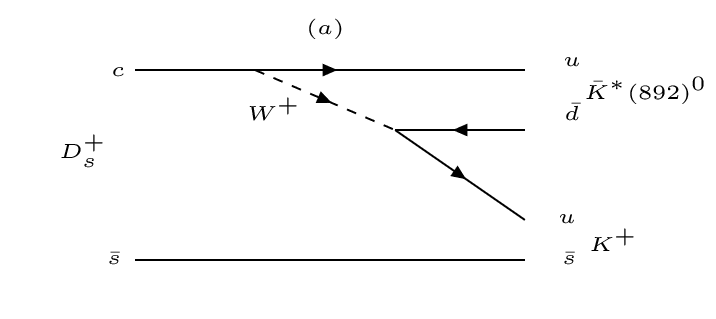
\includegraphics[width=0.45\textwidth]{plot/Fa.PNG}
        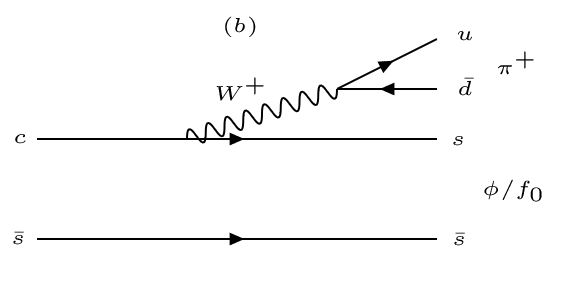
\includegraphics[width=0.45\textwidth]{plot/Fb.PNG}
        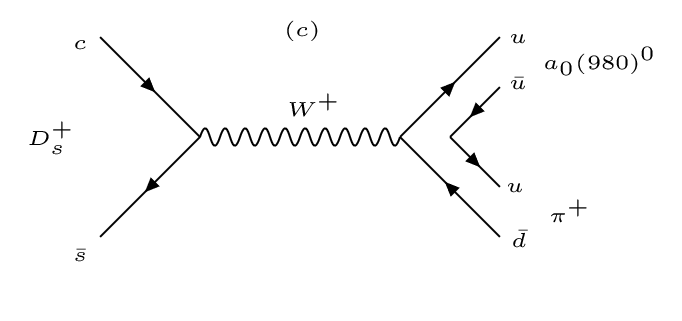
\includegraphics[width=0.45\textwidth]{plot/Fc.PNG}
        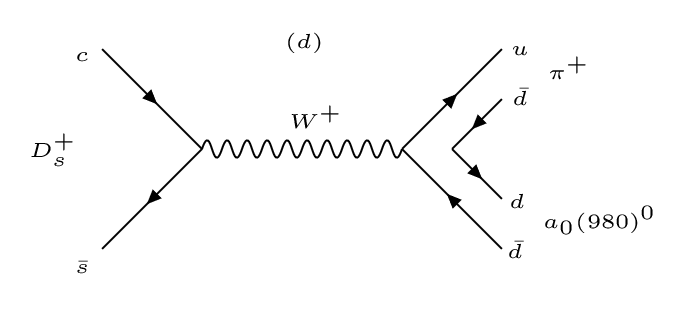
\includegraphics[width=0.45\textwidth]{plot/Fd.PNG}
        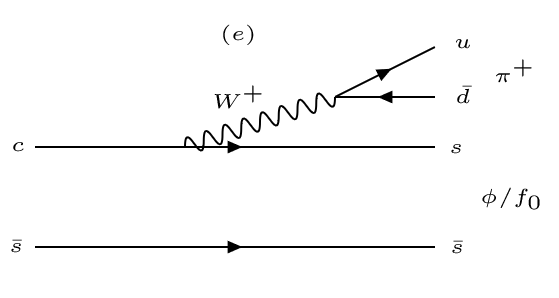
\includegraphics[width=0.45\textwidth]{plot/Fe.PNG}
        \caption{Main Feynman diagrams associated with $D_{s}^{+} \rightarrow K^{+}K^{-}\pi^{+}$ decay.}
        \label{Feynman-dia}
    \end{figure*}
    The main contribution comes from the diagram with an internal $W^{+}$ emission(Fig. \ref{Feynman-dia}(a) and Fig. \ref{Feynman-dia}(b)), that describes the $D_{s}^{+} \rightarrow \bar{K}^{*}(892)^{0}K^{+}$ decay, 
    and the diagram with an external $W^{+}$ emission(Fig. \ref{Feynman-dia}(e)), that describes the diagram $D_{s}^{+} \rightarrow \phi\pi^{+}/ f_{0}\pi^{+}$, 
    and the diagram with W-annihilation(Fig. \ref{Feynman-dia}(c) and Fig. \ref{Feynman-dia}(d)), that describes the decay $D_{s} \rightarrow a_{0}(980)^{0}\pi^{+}$.
}
    
\subsection{Amplitude analysis}
\par{
    Knowledge of the decay amplitude allows us to properly account for interference effects when measuring absolute hadronic branching fractions of $D_{s}$ mesons.
    Amplitude analysis of this decay can help us to understand the interference effects and so an amplitude analysis is necessary.
Below is the table of previous analyses of this decay channel.}

\begin{table}
    \caption{previous analyses of this decay channel.}
    \label{PreviousAnalyses}
    \begin{center}
        \begin{tabular}{cccc}
            \toprule\toprule
            Decay mode & Fit fraction(BABAR)  & Fit fraction(CLEO-c)  & Fit fraction(E687)\\
            \midrule
            $D_{s}^{+} \rightarrow \bar{K}^{*}(892)^{0}K^{+}$              & 47.9$\pm$0.5$\pm$0.5  & 47.4$\pm$1.5$\pm$0.4& 47.8$\pm$4.6$\pm$4.0 \\
            $D_{s}^{+} \rightarrow \phi(1020)\pi^{+}$                      & 41.4$\pm$0.8$\pm$0.5  & 42.2$\pm$1.6$\pm$0.3& 39.6$\pm$3.3$\pm$4.7 \\
            $D_{s}^{+} \rightarrow f_{0}(980)\pi^{+}/a_{0}(980)\pi^{+}$    & 16.4$\pm$0.7$\pm$2.0  & 28.2$\pm$1.9$\pm$1.8& 11.0$\pm$3.5$\pm$2.6 \\
            $D_{s}^{+} \rightarrow \bar{K}^{*}_{0}(1430)^{0}K^{+}$         & 2.4$\pm$0.3$\pm$1.0   & 3.9$\pm$0.5$\pm$0.5 & 9.3$\pm$3.2$\pm$3.2  \\
            $D_{s}^{+} \rightarrow f_{0}(1710)\pi^{+}$                     & 1.1$\pm$0.1$\pm$0.1   & 3.4$\pm$0.5$\pm$0.3 & 3.4$\pm$2.3$\pm$3.5  \\
            $D_{s}^{+} \rightarrow f_{0}(1370)\pi^{+}$                     & 1.1$\pm$0.1$\pm$0.2   & 4.3$\pm$0.6$\pm$0.5 & ...                  \\ 
            $\begin{matrix}\sum FF(\%)\end{matrix}$                          & 110.2$\pm$0.6$\pm$2.0 & 129.5$\pm$4.4$\pm$2.0 & 111.1\\
                \midrule
                $\chi^{2}/NDF$                                                  & $\frac{2843}{2305-14}=1.2$ & $\frac{178}{117}=1.5$ & $\frac{50.2}{33}=1.5$\\
                \midrule
                Events                                                         &$96307\pm369$          &$12226\pm22$  &$701\pm36$\\
                \bottomrule\bottomrule
            \end{tabular}
        \end{center}
    \end{table}


    From Table\ref{PreviousAnalyses}~\cite{2011BARBAR}, we can see an obvious difference of decay fraction of $f_{0}(980)\pi^{+}$ between BARBAR and CLEO-c. E687 used about 700 events and the E687 model did not take $f_{0}(1370)\pi^{+}$ into account. For CLEO-c, about 14400 events with purity about 84.9\% were selected with single tag method. The analysis of BARBAR used about 100000 events with purity about 95\%. In this analysis with double tag method, we can get a nearly background free data sample, that will be good to perform the amplitude analysis.
}

    \iffalse
    As shown in Fig. \ref{fig:lambc_cs} and Figure~\ref{fig:lambc_cs_bes3}, at the energy of 4.6\,GeV, cross section of producing $\lambdacp\lambdacm$ pair in $\ee$ collisions is $\sigma(\ee\to\lambdacp\lambdacm)=0.38\pm0.13\,\rm{nb}$ measured by BELLE~\cite{Pakhlova:2008vn} and $\sigma(\ee\to\lambdacp\lambdacm)=0.253\pm0.023\,\rm{nb}$ measured by BESIII~\cite{Weiping:lineshape}.\\

    %%%%%%%%%%%%%%%%%%%%%%%%%%%%


    %%%%%%%%%%%%%%%%%%%%%%%%%%%%
    \begin{figure*}[h]
        \centering
        \includegraphics[width=0.45\textwidth]{bes3_lineshape.eps}
        \caption{Cross sections of $\ee\to\lambdacp\lambdacm$ measured by BESIII.}
        \label{fig:lambc_cs_bes3}
    \end{figure*}
    %%%%%%%%%%%%%%%%%%%%%%%%%%%%%
    \fi


\section{Data Set and Monte Carlo Samples}
We use 3.195 ${\rm fb}^{-1}$ data set collected at $E_{cm} = 4.178$ GeV by BES\uppercase\expandafter{\romannumeral3} detector in 2016. Both data sample and Monte Carlo samples are reconstructed under BOSS7.0.3. 
All samples were generated with run-dependent $E_{cm}$~\cite{DocDB 580-v1}, except for the Bhabha, $\mu$-pair and Two-photon fusion events.
For these three types of events, we used a constant $E_{cm}$ at 4178.37 MeV, which is twice of a luminosity-weighted average of the measured beam energy in the center-of-mass frame. 
Total 40 rounds of generic MC with each round equaling to data size are used for background study, tag efficiencies estimation (rounds 01-30) and input-output check for branching fraction measurement (rounds 31-40). 
They are available at
/besfs3/offline/data/703-1/4180/mc/.
For each round of generic MC, the detail components and corresponding size of each Monte Carlo sample are given in Table~\ref{tab:genMC}.
\begin{table}[htp]
\begin{center}
\caption{Component and corresponding sizes, assume luminosity = 3195/pb.
    The cross sections of the open charm components except  $D_{s}^{+}D_{s}^{-}$ ~\cite{DocDB 580-v1} and $D_{s}^{*+}D_{s}^{-}$ ~\cite{preliminary} are measured by CLEO-c~\cite{PRD80-072001}.
}
\begin{tabular}{c|c|c|c} \hline
Component        & cross section (pb) & Size (M) & directory \\ \hline
$D^{0}D^{0}$     &        179         & 0.5719  &  D0D0 \\
$D^{+}D^{-}$     &        197         & 0.6294  &  DpDm \\
$D^{*0}D^{0}$    &       1211         & 3.8691  &  DST0D0 \\
$D^{*+}D^{-}$    &       1296         & 4.1407  &  DSTpDm \\
$D^{*0}D^{*0}$   &       2173         & 6.9427  &  DST0DST0 \\
$D^{*+}D^{*-}$   &       2145         & 6.8533  &  DSTpDSTm \\
    $D_{s}^{+}D_{s}^{-}$ ~\cite{DocDB 580-v1}&      7         & 0.0225  &  DsDs \\
    $D_{s}^{*+}D_{s}^{-}$ ~\cite{preliminary}&   961         & 3.0700  &  DsSTDs \\
\hline
$DD^{*}\pi^{+}$  &        383         & 1.2237  &  DDSTPIp \\
$DD^{*}\pi^{0}$  &        192         & 0.6134  &  DDSTPI0 \\
$DD\pi^{+}$      &         50         & 0.1598  &  DDPIp \\
$DD\pi^{0}$      &         25         & 0.0799  &  DDPI0 \\
\hline
Component        &  cross section (nb)& Size (M) & directory\\ \hline
$q\bar{q}$       &       13.8         & 44.0910  & qq \\
$\gamma J/\psi$  &        0.40        &  1.2780  & RR1S \\
$\gamma \psi(2S)$&        0.42        &  1.3419  & RR2S \\
$\gamma \psi(3770)$ &     0.06        &  0.1917  & RR3770 \\
$\tau \tau$      &        3.45        & 11.0228  & tt \\
$\mu \mu$        &        5.24        & 16.7418  & mm \\
$ee$             &      423.99        & 13.5465(0.01$\times$)  & ee\\
Two-photon\ fusion  &        1.7         &  5.4315   & TwoGam \\
HCT              &        0.10178     &  0.3252   & HCT \\
\hline
\end{tabular}
\label{tab:genMC}
\end{center}
\end{table}

%%\begin{table}[htp]
%\begin{center}
%\caption{Component and corresponding observed cross section (output from ConExc) for
%charmonium hadronic transition (HCT) processes.}
%\begin{tabular}{c|c|c|c} \hline
%Mode   & Final state       & Observed cross section & Referee of input line shape    \\
%index  &                   & @ 4180 MeV (nb)        &                                \\
%\hline 
%79 &   $\pi^0 \pi^0 \psi(2S)$  & 0.00342491         & BELLE  PRL99, 142002 (2007)    \\
%91 &   $\pi^+ \pi^- \psi(2S)$  & 0.00684981         & BELLE  PRL99, 142002 (2007)    \\
%80 &   $\eta J/\psi$           & 0.0321958          & BELLE  PRD87, 051101(R) (2013) \\
%81 &   $\pi^+ \pi^- h_c$       & 0.0122136          & BESIII PRL111,242001 (2013)    \\
%82 &   $\pi^0 \pi^0 h_c$       & 0.00610681         & BESIII PRL111,242001 (2013)    \\
%83 &   $K^+ K^- J/\psi$        & 0.000671349        & BELLE  PRD77, 011105(R) (2008) \\
%84 &   $K_S^0 K_S^0 J/\psi$    & 0.000167837        & BELLE  PRD77, 011105(R) (2008) \\
%90 &   $\pi^+ \pi^- J/\psi$    & 0.026767           & BELLE  PRL99, 182004 (2007)    \\
%99 &   $\pi^0 \pi^0 J/\psi$    & 0.0133835          & BELLE  PRL99, 182004 (2007)    \\
%\hline
%sum &                          & 0.101780616       &                                 \\
%\hline
%\end{tabular}
%\label{tab:HCT}
%\end{center}
%\end{table} 


For the Signal MC, we generate the signal events with one $D_{s}$ decaying to signal mode using the generator ``DIY'', in which the parameters are obtained from the fit to data. Phase space (PHSP) MC and Signal MC are used in MC integration required for the amplitude fit. The Signal MC is also used in the input/output check.

%%%%%%%%%%%%%%%%%%%%%%%%%%%%


%%%%%%%%%%%%%%%%%%%%%%%%%%%%


\section{Event Selection}
At $E_{cm} = 4.178 GeV$, pairs of $D_{s}D_{s}^{*}$ are produced,  and the $D_{s}^{*}$ decays to either $D_{s}\gamma$ or $D_{s}\pi^{0}$.  We use double tag method to select our signal events.


\subsection{Tracking, PID, $\pi^{0}/\eta^{(')}$ and $K_{S}^{0}$ Rconstruction }
$D_{s}$ candicates are built from $K^{\pm}$, $\pi^{\pm}$, $\pi^{0}/\eta^{(0)}$ and $K_{S}^{0}$. The selections of the particles to build $D_{S}$ candicates are performed with DTagAlg-00-01-05 package with the default setting, which are summarized below.

\begin{itemize}
	\item Tracking:
		\begin{itemize}
			\item[-] The properties of charged tracks are determined based on the MDC information. Charged track candidates must satisfy:
				\begin{itemize}
					\item[-] $|cos\theta| < 0.93$.
					\item[-] $|dr| < \boldmath 1cm$ and $|dz| < \boldmath 10cm$,

						where $|dr|$ and $|dz|$ are defined as the one reconstructed minus the interaction point.
				\end{itemize}
		\end{itemize}
	\item Particle ID:
		\begin{itemize}
			\item[-] Charged tracks are identified as pion or kaon with Particle Identification (PID), which is implemented by combing the information of the energy loss (dE/dx) in MDC and the time-of-flight measured from
				the TOF system. Kaon and Pion are identified with the requirements that 
				\begin{itemize}
					\item[-] $\emph{Prob(K)} > 0.00$ and $\emph{Prob(K)} > \emph{Prob($\pi$)}$ for \emph{K},
					\item[-] $\emph{Prob($\pi$)} > 0.00$ and $\emph{Prob($\pi$)} > \emph{Prob(K)}$ for \emph{$\pi$},
						where \emph{Prob(X)} is the probability of hypothesis X, X can be \emph{$\pi$} or \emph{K}.
				\end{itemize}
		\end{itemize}
	\item $\pi^{0}/\eta$ selection: $\pi^{0}$ candidates are reconstructed through $\pi^{0} \rightarrow \gamma\gamma$ with package of PioEtaToGGRecAlg.
		

		The photons are reconstructed as energy showers on the EMC. We require:
		\begin{itemize}
			\item[-] Minimum energy for barrel showers( $|cos\theta| < 0.8$): $E_{min} >25MeV/c^{2}$,
			\item[-] Minimum energy for endcap showers( $0.86 < |cos\theta| < 0.92$): $E_{min} >50MeV/c^{2}$,
			\item[-] Shower within other $|cos\theta|$ regions are rejected.
			\item[-] EMC time requirements for events with at least one charged track detected: $0 \le t \ge 14 $(50ns),
		\end{itemize}

		Then we perform a constrained fit on the photon pairs to the nominal $\pi^{0}/\eta$ mass and require:
		\begin{itemize}
			\item[-] The unconstrained invariant mass for $\pi^{0}$: $0.115 < M(\gamma\gamma) < 0.015 GeV/c^{2}$,
			\item[-] The unconstrained invariant mass for $\eta: 0.490 < M(\eta) < 0.580 GeV/c^{2}$,
			\item[-] Mass fit: $\chi_{1c}^{2} < 30$.
		\end{itemize}
	\item $\eta^{'}$ selection: The $\eta^{'}$ candidates are reconstructed with $\pi^{+}\pi^{-}\eta$, the invariant mass for $\pi^{+}\pi^{-}\eta$ is required to fall into the range of $[0.938, 0.978] GeV^{2}$.
	\item $K_{S}^{0}$ selection: $K_{S}^{0}$ candidates are reconstructed using VeeVertexAlg package with two opposite charged tracks with requiring:
		\begin{itemize}
			\item[-] $|cos\theta| < 0.93$
			\item[-] $|dz| < 20 \emph{cm} $
		\end{itemize}

		For each pair of tracks, a constrained vertex fit is performed and the track parameters' results are used to get the invariant mass $M(K_{S}^{0})$. Then the decay length of $K_{S}^{0}$ is obtained with second vertex 
		fit by the SecondVertexFit package. For $K_{S}^{0}$ selection, we require:
		\begin{itemize}
			\item[-] $0.487GeV/c^{2} < M(K_S^{0}) < 0.511 GeV/c^{2}$.
			\item[-] Significance of the $K_{S}^{0}$ decay lenght has two standard deviations.
		\end{itemize}

	\item $D_{s}$ selection: According to the MC study on $D_{s}$ reconstruction (BESS\uppercase\expandafter{\romannumeral3}-DocDB-380), the $D_{s}$ candidates fall into the mass window of $1.90 < m_{D_{s}} < 2.03 GeV/c^{2}$ and 
		the corresponding $M_{rec}$ satisfied $2.051 < M_{rec} < 2.180 GeV/c^{2}$ are retained for further study. In which, the definition of $M_{rec}$ is
		\begin{equation}
			M_{rec} = \sqrt{(E_{cm} - \sqrt{p_{D_{s}}^{2} + m_{D_{s}}^{2})^{2}} - |\vec p_{cm} - \vec p_{D_{s}} | ^{2}} \; , \label{con:inventoryflow}
		\end{equation}
		where $E_{cm}$ is the energy of initial state, calculated from the beam energy ~\cite{DocDB 580-v1}, $\vec p_{D_{s}}$ is the momentum of $D_{s}$ candidate, $m_{D_{s}}$ is $D_{s}$ mass quoted from PDG ~\cite{PDG} and $\vec p_{cm}$ and $\vec p_{D_{s}}$ are four-momentum of initial state and the decay products of a $D_{s}$ candidate, respectively.
\end{itemize}

\subsection{Single Tag Selection}
As $D_{s}^{+}$ and $D_{s}^{-}$ should appear in pairs, so we can use double tag method to select signal events. After $K^{\pm}$, $K_S^{0}$, $\pi^{\pm}$ and $\gamma$ are identified, hadronic $D_{s}$ decays can be reconstructed with the DTag package. 8 tag modes are used:

$D_{s}^{-} \rightarrow K^{+}K^{-}\pi^{-}$, $D_{s}^{-} \rightarrow K_{S}^{0}K^{-}$, $D_{s}^{-} \rightarrow K_{S}^{0}K^{-}\pi^{+}\pi^{-}$, $D_{s}^{-} \rightarrow K^{-}\pi^{+}\pi^{-}$, $D_{s}^{-} \rightarrow K_{S}^{0}K^{+}\pi^{-}\pi^{-}$, $D_{s}^{-} \rightarrow \pi^{+}\pi^{-}\pi^{-}$, $D_{s}^{-} \rightarrow \eta^{'}_{\pi^{+}\pi^{-}\eta_{\gamma\gamma}}$, $D_{s}^{-} \rightarrow K^{+}K^{-}\pi^{-}\pi^{0}$.


Before selecting the best candidate,  we vote the candidates with $\pi^{\pm}$($\pi^{0}$) whose momentum is less than $0.1GeV$ to remove soft $\pi^{\pm}$($\pi^{0}$) from $D^{*}$ decays.


For every candidate of $D_{s}$ decays, all tracks at signal side and tag side as well as gamma from $D_{s}^{*}$ are added to apply kinematic fitting. 5 constrains are added in kinematic fitting: four-momentum of $D_{s}D_{s}^{*}$, mass of $D_{s}^{*}$. Then we select the candidate with minmimum $\chi_{5c}^{2}$.  

The candidates satisfy:
\begin{itemize}
	\item[-] $1.95GeV < m_{sig} < 1.985GeV$
	\item[-] $1.95GeV < m_{tag} < 1.985GeV$
	\item[-] $\chi_{5c}^{2} < 50 $
\end{itemize}
are retained for amplitude analysis, where $m_{sig}$ and $m_{tag}$ refer to mass of $D_{s}$ at signal side and tag side respectively.

\subsection{Background Analysis}
We use generic MC to estimate the background. The background and signal shape of generic MC is shown in Fig.\ref{background and signal distribution}. According to the luminosities of the data and the generic MC, after scaling the background sample to the data size, the background yiels in Signal region is 11.8. Then the fit to the signal $D_{s}$ invariant mass ($m_{sig}$) spectrum gives the background yield in Signal region is $11.3 \pm 3.9$, shown as in Fig.\ref{mDs_fit}.  The background level in MC is then consistent with the data. In the fit, the signal shape is the MC shape convoluted with a Gaussian function and the background is the MC shape. 

\begin{figure*}[htbp]
 \centering
 \mbox{
  %\vskip -1.5cm
  \begin{overpic}[width=0.96\textwidth]{plot/mDs.eps}
  \end{overpic}
 }
 \caption{The background (a) and signal (b) distributions from generic MC after selection }
\label{background and signal distribution}
\end{figure*}

\begin{figure*}[h]
 \centering
 \mbox{
  %\vskip -1.5cm
  \begin{overpic}[width=0.48\textwidth]{plot/mDs_fit.eps}
  \end{overpic}
 }
 \caption{The fit to $m_{sig}$ for data after selections, the area between the purple arrows is the signal area of the sample for the amplitude analysis. }
\label{mDs_fit}
\end{figure*}


%%%%%%%%%%%%%%%%%%%%%%%%%%%%


%%%%%%%%%%%%%%%%%%%%%%%%%%%%


\section{Model Independent Partial Wave Analysis}
\par{In the $K^{+}K^{-}$ threshold both $a_{0}(980)$ and $f_{0}(980)$ can be present, and both resonances have very similar parameters which suffer from large uncertainties. In this section we obtain model-independent information on the $K^{+}K^{-} S$ wave by performing a MIPPPWA(model indendent partial wave analysis) in the  $K^{+}K^{-}$ threshold region.}
\subsection{Signal Candidate Selection}
\label{MIPWASelection}
\par{
    After the selection in Set.\ref{ST-selection}, we continue to select signals for model independent partial wave analysis.
    As MIPWA need more data events, we do not requre $D_{s}^{+}$ and $D_{s}^{-}$ appear in pairs. 
Before selecting the best candidate,  we vote the candidates with $\pi^{\pm}$($\pi^{0}$) whose momentum is less than $0.1GeV$ to remove soft $\pi^{\pm}$($\pi^{0}$) from $D^{*}$ decays.
For every candidates of $D_{s}$ decays, all tracks at signal side are added to apply kinematric fitting. Only mass of $D_{s}$ from signal side is constrained.Then we select the candidate with minimum $\chi_{1c}^{2}$.
}
\subsection{Background Analysis}
In order to further suppress the background, the multiple-variable analysis (MVA) is used. We train MVA methos separately with different sets of variables for the two event categories depending on the $D_{s}^{+}$ origin. 
Sideband region used below is defined as the region of  $1.90 < M(D_{s}) < 1.952 GeV$ and   $1.985 < M(D_{s}) < 2.03 GeV$, $M(D_{s})$ is the invariant mass of $D_{s}$.
And the signal region is $1.952 < M(D_{s}) < 1.985 GeV$.
These two categories of events are selected in a $M_{rec}-\Delta{M}$ 2D plane shown in Fig.\ref{2DAll}:

\begin{figure*}[h]
 \centering
 \mbox{
  %\vskip -1.5cm
  \begin{overpic}[width=0.48\textwidth]{plot/2DAll.png}
  \end{overpic}
 }
 \caption{Two dimensional plane of ${M_{rec}}$ versus ${\Delta{M} \equiv M(D_{s}^{+}\gamma) - M(D_{s}^{+})}$ from the simulated ${D_{s}^{+} \rightarrow K^{+}K^{-}\pi^{+}}$ decyas. The red(green) dashed lines mark the mass window for the $D_{s}^{+}$ Cat. \#0( Cat. \#1) around the $M_{rec}$($\Delta{M}$) peak. }
\label{2DAll}
\end{figure*}



\begin{itemize}
    \item Cat. \#0: Direct $D_{s}^{+}$. We use the following variables whose distributions for signal and background are shown in Fig.\ref{Cat0Variables},
        \begin{itemize}
            \item[1. ] $M_{rec}$,
            \item[2. ] $P_{rest}$, defined as the total momentum of the tracks and neutrals in the rest of event (not part of the $D_{s}^{+} \rightarrow K^{+}K^{-}\pi^{+}$ candidate),
            \item[3. ] $E_{\gamma}$, defined as the energy of gamma from $D_{s}^{*}$.
        \end{itemize}
        From Fig. \ref{Cat0Variables}(generic MC) and Fig.\ref{cat0_data}(data), we can see that the corresponding distributions of these variables of data and generic MC are roughly consistent.
        

    \item Cat. \#1: Indirect $D_{s}^{+}$.
        We use the following variables whose distributions for signal and background are shown in Fig.\ref{Cat1Variables},
        \begin{itemize}
            \item[1. ] $\Delta{M}$,
            \item[2. ] $M_{rec}^{'}$, defined as $M_{rec}^{'} = \sqrt{ {(E_{cm}  - \sqrt{p_{D_{s}\gamma}^{2} + m_{D_{s}^{*}}^{2}}) }^{2} - p_{D_{s}\gamma}^{2}}$, with $p_{D_{s}\gamma}$ as the momentum of the $D_{s}\gamma$ combination, $m_{D_{s}^{*}}$ as the nominal ${D_{s}^{*}}$ mass,
            \item[3. ] $N_{tracks}$, defined as the total number of tracks and neutrals in an event.
        \end{itemize}
        From Fig. \ref{Cat1Variables}(generic MC) and Fig.\ref{cat1_data}(data), we can see that the corresponding distributions of these variables of data and generic MC are roughly consistent.
\end{itemize}


\begin{figure*}[h]
 \centering
 \mbox{
  %\vskip -1.5cm
  \begin{overpic}[width=0.99\textwidth]{plot/Cat0Variables.png}
  \end{overpic}
 }
 \caption{ For event Cat. \#0,  distributions of MVA variables from simulated signal decays and background events.}
\label{Cat0Variables}
\end{figure*}

\begin{figure*}[!htbp]
 \centering
 \includegraphics[width=0.99\textwidth]{plot/cat0_sig.eps}
 \includegraphics[width=0.99\textwidth]{plot/cat0_sb.eps}
 \caption{The distribution(Cat. \#0) of these three observables ((a) and (d)) $M_{rec}$, ((b) and (e)) $P_{rest}$ and  ((c) and (f)) $E_{\gamma}$ for( (a), (b) and (c)) Signal and ( (d), (e) and (f)) Sideband regions from data are shown.}
\label{cat0_data}
\end{figure*}

\begin{figure*}[h]
 \centering
 \mbox{
  %\vskip -1.5cm
  \begin{overpic}[width=0.99\textwidth]{plot/Cat1Variables.png}
  \end{overpic}
 }
 \caption{ For event Cat. \#1,  distributions of MVA variables from simulated signal decays and background events.}
\label{Cat1Variables}
\end{figure*}

\begin{figure*}[!htbp]
 \centering
 \includegraphics[width=0.99\textwidth]{plot/cat1_sig.eps}
 \includegraphics[width=0.99\textwidth]{plot/cat1_sb.eps}
 \caption{The distribution(Cat. \#1) of these three observables ((a) and (d)) $M_{rec}$, ((b) and (e)) $P_{rest}$ and  ((c) and (f)) $E_{\gamma}$ for( (a), (b) and (c)) Signal and ( (d), (e) and (f)) Sideband regions from data are shown.}
\label{cat1_data}
\end{figure*}

\par{As the results shown in Fig.\ref{Overtrain}, this BDTG training and test samples are well matched. For event Cat. \#0 ( Cat. \#1 ), the sample with BDTG value larger than 0.33(0.65) is retained for further study. 
    
\begin{figure*}[h]
    \centering
    \mbox{
        %\vskip -1.5cm
        \begin{overpic}[width=0.48\textwidth]{plot/Cat0Overtrain.eps}
        \end{overpic}
    }
    \mbox{
        %\vskip -1.5cm
        \begin{overpic}[width=0.48\textwidth]{plot/Cat1Overtrain.eps}
        \end{overpic}
    }
    \caption{ The comparisions between the training and test samples. The plot at left(right) is the comparision of Cat. \#0 (Cat. \#1).}
    \label{Overtrain}
\end{figure*}
    
   
    After applying the BDTG requirement, the background shows no obviously peak around the region of [1.95, 1.982] $GeV$ (Signal region), which are shown in Fig.\ref{MIPWA-ST-BS}.  The fit to the signal $D_{s}$ invariant mass ($M_{D_{s}^{2}}$) spectrum gives the background yield in Signal region is $73.6\pm18.7$, shown as in Fig.\ref{MIPWA-ST}. In the fit, the signal shape is the MC shape convoluted with a Gaussian function and the background is described with $1^{st}$-order Chebychev polynomial.

    \begin{figure*}[h]
        \centering
        \mbox{
            %\vskip -1.5cm
            \begin{overpic}[width=0.48\textwidth]{plot/MIPPWA-sig.eps}
            \end{overpic}
        }
        \mbox{
            %\vskip -1.5cm
            \begin{overpic}[width=0.48\textwidth]{plot/MIPPWA-bkg.eps}
            \end{overpic}
        }
        \caption{ The signal and background distributions from generic MC after BDTG requirement.}
        \label{MIPWA-ST-BS}
    \end{figure*}

}

\begin{figure*}[h]
 \centering
 \mbox{
  %\vskip -1.5cm
  \begin{overpic}[width=0.8\textwidth]{plot/MIPPWA-ST.eps}
  \end{overpic}
 }
 \caption{The fit to the signal $D_{s}$ invariant mass ($M_{D_{s}}$) spectrum after BDTG requirement, the area between the pink arrows is the signal area of the sample for MIPWA. }
\label{MIPWA-ST}
\end{figure*}

\par{
The projections of the "Sideband"( $1.90 < M(D_{s}) < 1.95 GeV$ and   $1.985 < M(D_{s}) < 2.03 GeV$) from data and generic MC after signal events removed are shown in Fig.\ref{MIPWA-Sideband}. The corresponding plots agree well.} 



\begin{figure*}[h]
    \centering
    \mbox{
        %\vskip -1.5cm
        \begin{overpic}[width=0.3\textwidth]{plot/MIPPWA-m12.eps}
        \end{overpic}
    }
    \mbox{
        %\vskip -1.5cm
        \begin{overpic}[width=0.3\textwidth]{plot/MIPPWA-m13.eps}
        \end{overpic}
    }
    \mbox{
        %\vskip -1.5cm
        \begin{overpic}[width=0.3\textwidth]{plot/MIPPWA-m23.eps}
        \end{overpic}
    }
    \caption{ The projections of $m(K^{+}K^{-})$, $m(K^{-}\pi^{+})$, $m(K^{+}\pi^{+})$ from "Sideband" for data(dots with error bars) and generic MC after signal events removed (red histogram) after BDTG requirement.}
    \label{MIPWA-Sideband}
\end{figure*}

\par{Thus the generic MC sample with signal events removed is used to subtract the background in MIPWA.
}


\subsection{MIPWA method}
\par{Let N be the number of events for a given mass interval $I=[m_{K^{+}K^{-}}; m_{K^{+}K^{-}} + dm_{K^{+}K^{-}}]$. We write the corresponding angular distributions in terms of the appropriate spherical harmonic functions as
    \begin{equation}
        \frac{dN}{d\cos\theta} = 2\pi\sum_{k=0}^L\left\langle Y_{k}^{0}\right\rangle Y_{k}^{0}(\cos\theta),\label{expansion}
    \end{equation}
    where $L - 2 \ell_{max}$, and $\ell_{max}$ is the maximum orbital angular momentum quantum number required to describe the $K^{+}K^{-}$ system at $m_{K^{+}K^{-}}$ (e.g. $\ell_{max}$ =1 for S-, P-wave description); $\theta$ is the angle between the $K^{+}$ direction in the $K^{+}K^{-}$ system in the $D_{s}^{+}$ rest frame. The normalizations are such that
    \begin{equation}
        \int_{-1}^{1}Y_{k}^{0}(\cos\theta)Y_{j}^{0}(\cos\theta), d\cos\theta  = \frac{\delta_{kj}}{2\pi},\label{sh-normalizations}
    \end{equation}
    and it is  assumed that the distribution $\frac{dN}{d\cos\theta}$ has been efficiency corrected and background subtracted.
    Using this orthogonality condition, the coefficiencies in the expansion are obtained from 
    \begin{equation}
        \left\langle Y_{k}^{0} \right\rangle = \int_{-1}^{1} \frac{dN}{d\cos\theta} d\cos\theta,\label{expansion-coefficiencies}
    \end{equation}
    where the intergral is given, to a good approximiation, by $\sum_{n=1}^{N}Y_{k}^{0}(\cos\theta_{n})$, where $\theta_{n}$ is the value of $\theta$ for the $n$-th event.
    
    Fig.\ref{Y0} shows the $K^{+}K^{-}$ mass spectrum up to 1.15 GeV weighted by $Y_{k}^{0}(\cos\theta) = \sqrt{(2k+1)/(4\pi)}P_{k}(\cos\theta)$ for k=0, 1, and 2, where $P_{k}$ is the Legendre ploynomial function of orkder $k$. These distributions are corrected for efficiency and phase space, and background is subtracted using background from generic MC after BDTG requirement.
    
    The number of events N for the mass interval $I$ can be expressed also in terms of the partial-wave amplitudes describing the $K^{+}K^{-}$ system. Assuming that only S- and P-wave amplitudes are necessary in this limited region, we can write:
    \begin{equation}
        \frac{dN}{d\cos\theta} = 2\pi\left|SY_{0}^{0}(\cos\theta) + PY_{1}^{0}(\cos\theta)\right|^{2}.\label{SP-distribution}
    \end{equation}
    By comparing Eqa. \ref{expansion} and \ref{SP-distribution}, we obtain 
    \begin{equation}
        \begin{array}{lr}
            \sqrt{4\pi}\left\langle Y_{0}^{0}\right\rangle = \left|S\right|^{2} + \left|P\right|^{2}, &\\ 
            \sqrt{4\pi}\left\langle Y_{2}^{0}\right\rangle = \frac{2}{\sqrt{5}}\left|P\right|^{2}, &
        \end{array}\label{SP-RES} 
    \end{equation}

}

\begin{figure*}[h]
    \centering
    \mbox{
  %\vskip -1.5cm
  \begin{overpic}[width=0.9\textwidth]{plot/Y0.eps}
  \end{overpic}
 }
 \caption{ $K^{+}K^{-}$ mass spectrum in the threshold region weighted by (a) $Y_{0}^{0}$, (b) $Y_{1}^{0}$ and (c) $Y_{2}^{0}$, corrected for efficiency and phase space, and background subtracted. }
\label{Y0}
\end{figure*}

\par{The above system of equations can be solved in each interval of $K^{+}K^{-}$ invariant mass for $\left|S\right|$ and $\left|P\right|$ and the resulting distributions are shown in Fig.\ref{SP}.  
}

\begin{figure*}[h]
    \centering
    \mbox{
  %\vskip -1.5cm
  \begin{overpic}[width=0.9\textwidth]{plot/SP.eps}
  \end{overpic}
 }
 \caption{ Squared (a) S- and (b) P-wave amplitudes}
 \label{SP}
\end{figure*}

\subsection{S-wave parameterization at the $K^{+}K^{-}$ threshold}
\label{MIPPWA-RES}
\par{We empirically parameterize the $f_{0}(980)$ with the following function:
    \begin{equation}
        A_{f_{0}(980) / a_{0}(980)} = \frac{1}{m_{0}^{2} - m^{2} -im_{0}\Gamma_{0}\rho_{KK}}, \label{a0980-RBW}
    \end{equation}
    where $\rho_{KK} = 2p/m$, and obtain the flollowing parameter values:
    \begin{equation}
        \begin{array}{lr}
            m_{0} = (0.919 \pm 0.006_{stat}) GeV, &\\
            \Gamma_{0} = (0.272 \pm 0.040_{stat}) GeV. &
        \end{array}\label{S-wave parameters} 
    \end{equation}


    The errors are statistical only. The fit result are shown in Fig.\ref{FitSWave}.
    
    \begin{figure*}[h]
        \centering
        \mbox{
            %\vskip -1.5cm
            \begin{overpic}[width=0.8\textwidth]{plot/Fit-SWave.eps}
            \end{overpic}
        }
        \caption{ Fit of squared S-wave amplitudes. the curves result from the fit described in the text.}
        \label{FitSWave}
    \end{figure*}
}



\section{Amplitude Analysis}
\label{Amplitude-Analysis}
\subsection{Event Selection}
\label{AASelection}
\par{
    After $K^{\pm}$, $K_S^{0}$, $\eta$, $\eta^{'}$, $\pi^{\pm}$ and $\pi^{0}$ are identified in Sec.~\ref{ST-selection}, hadronic $D_{s}$ decays can be reconstructed with the DTag package. 
    Eight tag modes are used:

$D_{s}^{-} \rightarrow K^{+}K^{-}\pi^{-}$, $D_{s}^{-} \rightarrow K_{S}^{0}K^{-}$, $D_{s}^{-} \rightarrow K_{S}^{0}K^{-}\pi^{+}\pi^{-}$, $D_{s}^{-} \rightarrow K^{-}\pi^{+}\pi^{-}$, $D_{s}^{-} \rightarrow K_{S}^{0}K^{+}\pi^{-}\pi^{-}$, $D_{s}^{-} \rightarrow \pi^{+}\pi^{-}\pi^{-}$, $D_{s}^{-} \rightarrow \eta^{'}_{\pi^{+}\pi^{-}\eta_{\gamma\gamma}}$, $D_{s}^{-} \rightarrow K^{+}K^{-}\pi^{-}\pi^{0}$.


With the tagged $D_{s}$ meson, the signal $D_{s}$ is reconstructed with the remaining good tracks. 
The momentum of $\pi^{\pm}$ $(\pi^{0})$ is required to be larger than $100\ {\rm MeV/c^{2}}$ to suppress the background of $D^{*} \rightarrow D\pi$.
Only the $D_{s}$ candidate with invariant mass falls into $[1.87, 2.06]$ GeV/$c^{2}$ are selected.

For every candidate of $D_{s}D_{s}^{*}$ decays, all tracks at signal side and tag side as well as gamma from $D_{s}^{*}$ are added to apply kinematic fitting. 
Five constrains are added in kinematic fitting: four-momentum of $D_{s}D_{s}^{*}$ and mass of $D_{s}^{*}$. 
If the combination of signal $D_{s}$ and $\gamma$ to form $D_{s}^{*}$ have a lower $\chi_{5C}^{2}$ than that of tagged $D_{s}$ and $\gamma$, the signal $D_{s}$ should come from the $D_{s}^{*}$ decay.
Otherwise, the signal $D_{s}$ should directly come from the intersection point.
Then we select the candidate with minimum $\chi_{5C}^{2}$.  

The candidates satisfy:
\begin{itemize}
    \item[-] $m_{sig}$ and $m_{tag}$ falls in the mass regions shown in Table~\ref{ST-mass-window}, 
	\item[-] $\chi_{5C}^{2} < 200 $, 
\end{itemize}
are retained for the amplitude analysis, where $m_{sig}$ and $m_{tag}$ refer to mass of $D_{s}$ at signal side and tag side respectively.
After the selection above, if we find both $D_{s}^{+} \rightarrow K^{+}K^{-}\pi^{+}$ and $D_{s}^{-} \rightarrow K^{+}K^{-}\pi^{-}$ modes in an event, both of them are taken as our signals.

In addition, we use the four momentum after applying kinematic fitting with the mass of signal $D_{s}$ constrained to PDG value and the five constrains above to perform amplitude analysis.

\begin{table}[htbp]
    \caption{ The mass windows for each tag mode. The mass windows use the results in Ref.~\cite{Doc-DB-630-v35} }
    \label{ST-mass-window}
    \begin{center}
        \begin{tabular}{cc}
            \toprule\toprule
            Tag mode & Mass window (GeV/$c^{2}$)  \\
            \hline
            $D_{s}^{-} \rightarrow K_{S}^{0}K^{-}$                          & [1.948, 1.991]    \\
            $D_{s}^{-} \rightarrow K^{+}K^{-}\pi^{-}$                       & [1.950, 1.986]    \\
            $D_{s}^{-} \rightarrow K^{+}K^{-}\pi^{-}\pi^{0}$                & [1.947, 1.982]    \\
            $D_{s}^{-} \rightarrow K_{S}^{0}K^{-}\pi^{+}\pi^{-}$            & [1.958, 1.980]    \\
            $D_{s}^{-} \rightarrow K_{S}^{0}K^{+}\pi^{-}\pi^{-}$            & [1.953, 1.983]    \\
            $D_{s}^{-} \rightarrow \pi^{-}\pi^{-}\pi^{+}$                   & [1.952, 1.984]    \\
            $D_{s}^{-} \rightarrow \pi^{-}\eta_{\pi^{+}\pi^{-}\eta_{\gamma\gamma}}^{'}$  & [1.940, 1.996]        \\
            $D_{s}^{-} \rightarrow K^{-}\pi^{+}\pi^{-}$                     & [1.953, 1.983]    \\
            \bottomrule\bottomrule
        \end{tabular}
    \end{center}
\end{table}

}

\subsection{Background Analysis}
We use generic MC to estimate the background. The background and signal shape of generic MC is shown in Fig.~\ref{background-and-signal-distribution}. 
By scaling the generic MC background sample to the data size based on the luminosities, the background yields in the signal region is 17.2. 
The fit to the signal $D_{s}$ invariant mass ($m_{sig}$) spectrum gives the background yield in the signal region is $18.1 \pm 5.1$, shown as in Fig.~\ref{mDs_fit}.  
The background level in generic MC is consistent with the data. In the fit, the signal shape is the MC shape convoluted with a Gaussian function and the background is the MC shape. 

\begin{figure*}[htbp]
 \centering
 \mbox{
  %\vskip -1.5cm
  \begin{overpic}[width=0.9\textwidth]{plot/bkg.eps}
  \end{overpic}
 }
 \caption{ The background and the signal shape of generic MC (round 01-40)}
\label{background-and-signal-distribution}
\end{figure*}

\begin{figure*}[htbp]
 \centering
 \mbox{
  %\vskip -1.5cm
  \begin{overpic}[width=0.48\textwidth]{plot/mDs.eps}
  \end{overpic}
 }
 \caption{The fit to $m_{sig}$ for data after selections, the area between the purple arrows is the signal area of the sample for the amplitude analysis.
     The signal shape (green line) is the MC shape convoluted with a Gaussian function and the background (red line) is the MC shape.
 }
\label{mDs_fit}
\end{figure*}

\subsection{Fit Method}
\par{The method used in the amplitude analysis is the same as the Ref.~\cite{Doc-DB-416-v30}. In this section, we briefly review the amplitude analysis method used in this analysis.
    
    The relative magnitudes and phases of the partial waves and the mass and width of intermediate resonances are determined by an unbinned maximum-likelihood fit to the data selected. The formulas are constructed with covariant tensors~\cite{covariant-tensors}.

    Since there are three final state particles, only one possible resonant state is allowed in any intermediate process. Thus the amplitude of the $n^{th}$ intermediate state ($A_{n}$) is,
    \begin{equation}
        A_{n} = P_{n}S_{n}F_{n}^{r}F_{n}^{D}, \label{base-amplitude}
    \end{equation}
    where $S_{n}$ and $F_{n}^{r(D)}$ are the spin factor and the Blatt-Weisskopf barriers of the intermediate state (the $D_{s}$ meson), respectively. $P_{n}$ is the propagator of the intermediate resonance. 

The total amplitude $M$ is then the coherent sum of the amplitudes of intermediate processes, $M=\begin{matrix}\sum c_{n}A_{n}\end{matrix}$, where $c_{n}=\rho_{n}e^{i\phi_{n}}$ is the corresponding complex coefficient. The magnitude $\rho_{n}$ and phase $\phi_{n}$ are determined by the amplitude analysis. 
    The signal probability density function (PDF) $f_{S}(p_{j})$ is given by 
    \begin{equation}
        f_{S}(p_{j}) = \frac{\epsilon(p_{j})\left|M(p_{j})\right|^{2}R_{3}(p_{j})}{\int \epsilon(p_{j})\left|M(p_{j})\right|^{2}R_{3}(p_{j})\,dp_{j}}, \label{signal-PDF}
    \end{equation}
    where $\epsilon(p_{j})$ is the detection efficiency parameterized in terms of the final four-momenta $p_{j}$. The index $j$ refers to the different particles in the final states. 
    $R_{3}(p_{j})$ is the standard element of the three-body phase space. 
    The normalization integral is determined by a MC integration,
    \begin{equation}
    \int \epsilon(p_{j})\left|M(p_{j})\right|^{2}R_{3}(p_{j})\,dp_{j} \approx \frac{1}{N_{MC}} \begin{matrix}\sum_{k_{MC}}^{N_{MC}} \frac{\left|M(p_{j}^{k_{MC}})\right|^{2}}{\left|M^{gen}(p_{j}^{k_{MC}})\right|^{2}}\end{matrix}, \label{MC-intergral}
    \end{equation}
    where $k_{MC}$ is the index of the $k_{MC}^{th}$ event of the MC sample and $N_{MC}$ is the number of the selected MC events.  
    $M^{gen}(p_{j})$ is the PDF used to generate the MC samples in MC integration.
    At the beginning, the PHSP MC are used in MC integration. $M^{gen}(p_{j})$ is a constant overall the phase space.
    Then with the result obtained from the fit to data, the signal MC is then generated and used in MC integration.
    In this analysis, a PHSP MC sample with about 6 million events and  a signal MC sample with about 2 million events are used in the normalization integral calculation using PHSP MC and signal MC, respectively.
    In the numerator of Eq.~\ref{signal-PDF}, $\epsilon(p_{j})$ is independent of the fitted variables, so it is regarded as a constant term in the fit.
    %In addition, the MC events used in Eq.~\ref{MC-integral} is the events passed the event selection the same as the data sample, we do not need to consider the detection efficiency in the fit.
    Considering the bias caused by particle identification (PID)~\cite{PID} and tracking~\cite{Tracking} efficiency differences between data and MC, we introduce $\gamma_{\epsilon}$ to correct this bias:
    \begin{equation}
        \gamma_{\epsilon} = \prod_{i} \frac{\epsilon_{i, data}(p_{i})}{\epsilon_{i, MC}(p_{i})}, \label{experimental-effect}
    \end{equation}
    where $i$ denotes the three daughter particles. 
    %The values of $\frac{\epsilon_{i, data}(p_{i})}{\epsilon_{i, MC}(p_{i})}$ used in this analysis are from the references and.

    Since there is only about $0.4\%$ background in the data sample, the contribution from the background is ignored in the likelihood calculation:
    \begin{equation}
    \ln{\mathcal{L}} = \begin{matrix}\sum_{k}^{N_{data}} \ln f_{S}(p_{j}^{k})\end{matrix},  \label{likelihood}
    \end{equation}
    where $N_{data}$ is the number of candidate events in data.


    \subsubsection{Propagator}
    \label{propagator}
    \par{
        For a decay process $a \rightarrow bc$, $s_{a/b/c}$ is denoted to be the invariant mass square of the particle a/b/c, $r_{a}=p_{b}-p_{c}$, and q is denoted as the magnitude of the momentum of daughter particle in the rest system of $a$
        \begin{equation}
            q=\sqrt{ \frac{(s_{a} + s_{b} + s_{c})^{2}}{4s_{a}} - s_{b}}. \label{base-q}
        \end{equation}

        The intermediate resonances $K^{*}(892)^{0}$, $\phi(1020)$, $f_{0}(1370)$ and  $f_{0}(1710)$ are parameterized as a relativistic Breit-Wigner (RBW) formula,
        \begin{equation}
            \begin{array}{lr}
                P = \frac{1}{(m_{0}^{2} - s_{a} ) - im_{0}\Gamma(m)}, &\\
                \Gamma(m) = \Gamma_{0}\left(\frac{q}{q_{0}}\right)^{2L+1}\left(\frac{m_{0}}{m}\right)\left(\frac{X_{L}(q)}{X_{L}(q_{0})}\right)^{2}, &
            \end{array}\label{RBW} 
        \end{equation}
        where $m_{0}$ and $\Gamma_{0}$ are the mass and the width of the intermediate resonances, and are fixed to the PDG values~\cite{PDG2018} except the mass and the width of $f_{0}(1370)$. 
        The mass and width of $f_{0}(1370)$ are fixed to 1350 MeV$/c^{2}$ and 265 MeV$/c^{2}$~\cite{para-f01370}, respectively..
        The value of $q_{0}$ in Eq.~\ref{RBW} is that of $q$ when $s_{a}=m_{0}^{2}$, $L$ denotes the angular momenta and $X_{L}(q)$ is defined as:
        \begin{equation}
            \begin{array}{lr}
                X_{L=0}(q) = 1,       &\\
                X_{L=1}(q) = \sqrt{\frac{2}{z^{2}+1}},       &\\
                X_{L=2}(q) = \sqrt{\frac{13}{z^{4}+3z^{2}+9}},       &\\
            \end{array}\label{XLQ} 
        \end{equation}
        where $z=qR$. The R is the effective radius of the intermediate state or $D_{s}$ meson and set to $3.0\ {\rm GeV}^{-1}$ for intermediate states and $5.0\ {\rm GeV}^{-1}$  for $D_{s}$ meson~\cite{Doc-DB-416-v30}, respectively.
        This value R is a typical value used by $D$ physics and we will also vary this value as a source of systematic uncertainties.

        $K^{*}_{0}(1430)^{0}$ is parameterized with Flatte formula:
        \begin{equation}
            P_{K^{*}_{0}(1430)^{0}}= \frac{1}{M^{2} - s - i(g_{1}\rho_{K\pi}(s) + g_{2}\rho_{\eta^{'}K}(s))}, \label{Flatte}
        \end{equation}
        where $s$ is the $K^{-}\pi^{+}$ invariant mass squared,  $\rho_{K\pi}(s)$ and $\rho_{\eta^{'}K}(s)$ are Lorentz invariant PHSP factor, and   $g_{1,2}$ are coupling constants to the corresponding final state. The parameters of $K^{*}_{0}(1430)^{0}$ are fixed to values measured by CLEO~\cite{CLEO-Flatte}. 
        For resonances $f_{0}(980)$ and $a_{0}(980)$, as is discussed in Sec.~\ref{f0-a0-discussion}, we use Eq.~\ref{S980-RBW} to describe the propagator and the values of parameters are fixed to the values in Eq.~\ref{S-wave parameters} obtained from the model independent partial wave analysis section (Sec.~\ref{MIPWA-RES}).
    }

    \subsubsection{Blatt-Weisskopf Barriers}{
        The Blatt-Weisskopf barriers are given by 
        \begin{equation}
            \begin{array}{lr}
                F_{n} = 1,       \ \ \ \ \ \ \ \ \ \ \ \   (S\ wave), &\\
                F_{n} = \sqrt{\frac{z_{0}^{2}+1}{z^{2}+1}},      \ \     (P\ wave), &\\
                F_{n} = \sqrt{\frac{z_{0}^{4}+3z_{0}^{2}+9}{z^{4}+3z^{2}+9}},   \ \      (D\ wave), &
            \end{array}\label{Blatt-Weisskopf barrier} 
        \end{equation}
        where $z_{0} = q_{0}R$. 
    }

    \subsubsection{Spin Factors}
    \par{
        As the limit of the phase space, we only consider the states with angular momenta no more than 2. 
        Considering a two-body decay, the spin projection operators are defined as  
        \begin{equation}
            \begin{array}{lr}
                P^{0}(a) = 1,   \ \ \ \ \ \  \ \ \ \ \ \  \ \ \ \ \ \ \ \ \ \ \ \        (S\ wave), &\\
                P^{(1)}_{\mu\mu^{'}}(a) = -g_{\mu\mu^{'}}+\frac{p_{a,\mu}p_{a,\mu^{'}}}{p_{a}^{2}},          (P\ wave), &\\
                P^{2}_{\mu\nu\mu^{'}\nu^{'}}(a) = \frac{1}{2}(P^{(1)}_{\mu\mu^{'}}(a)P^{(1)}_{\nu\nu^{'}}(a)+P^{(1)}_{\mu\nu^{'}}(a)P^{(1)}_{\nu\mu^{'}}(a))+\frac{1}{3}P^{(1)}_{\mu\nu}(a)P^{(1)}_{\mu^{'}\nu^{'}}(a),\           (D\ wave). &
            \end{array}\label{spin-projection-operators} 
        \end{equation}
       The covariant tensors are given by 
        \begin{equation}
            \begin{array}{lr}
                \tilde{t}^{(0)}(a) = 1, \ \ \ \ \ \  \ \ \ \ \ \   \ \ \ \ \ \ \ \ \ \       (S\ wave), &\\
                \tilde{t}^{(1)}_{\mu}(a) = -P^{(1)}_{\mu\mu^{'}}(a)r^{\mu^{'}},   \ \  \ \ \ \         (P\ wave), &\\
                \tilde{t}^{(2)}_{\mu\nu}(a) = P^{(2)}_{\mu\nu\mu^{'}\nu^{'}}(a)r^{\mu{'}}_{a}r^{\nu^{'}}_{a}, \           (D\ wave). &\\
            \end{array}\label{covariant-tensors} 
        \end{equation}
        The spin factor for $D_{s} \rightarrow aX$ and then $a \rightarrow bc$ is( $a$ refers to the intermediate resonance), 
        \begin{equation}
            \begin{array}{lr}
                S_{n} = 1,         \ \ \ \ \ \  \ \ \ \ \ \ \ \ \ \ \ \  \ \ \ \ \ \ \ \ (S\ wave), &\\
                S_{n} = \tilde{T}^{(1)\mu}(D_{s})\tilde{t}^{(1)}_{\mu}(a),\ \          (P\ wave), &\\
                S_{n} = \tilde{T}^{(2)\mu\nu}(D_{s})\tilde{t}^{(2)}_{\mu\nu}(a),\ \         (D\ wave), &
            \end{array}\label{spin-factor} 
        \end{equation}
        where the $\tilde{T}^{(1)\mu}(D_{s})$($\tilde{T}^{(2)\mu}(D_{s})$) and $\tilde{t}^{(1)}_{\mu}(a)$($\tilde{t}^{(2)}_{\mu}(a)$) have same definition as in Ref.~\cite{covariant-tensors}.
    }

}


\subsection{Fit Fraction}
\label{FF}
\par{
The fit fractions of the individual amplitudes are calculated according to the fit results and are compared to the other measurements. In the calculation, a PHSP MC with neither detector acceptance nor resolution is involved. The fit fraction for an amplitude is defined as
    \begin{equation}
    FF(n) = \frac{\begin{matrix}\sum_{k=1}^{N_{gen}} \left|A_{n}\right|^{2}\end{matrix}}{\begin{matrix}\sum_{k=1}^{N_{gen}} \left|M(p_{j}^{k})\right|^{2}\end{matrix}}, \label{Fit-Fraction-Definition}
    \end{equation}
    where $N_{gen} = 2000000$, is the number of the PHSP MC events at generator level. 

    To estimate the statistical uncertainties of the fit fractions, we repeat the calculation of fit fractions by randomly varying the fitted parameters according to the error matrix. 
    Then, for each amplitude , we fit the resulting distribution with a Gaussian function, whose width gives the corresponding statistical uncertainty.
}

\subsection{Fit Result}
\par{
    The Dalitz plot of $m^{2}(K^{+}K^{-})$ versus $m^{2}(K^{-}\pi^{+})$ is shown in Fig.~\ref{dalitz}. 
    In the plot, we can see a clear peak of $K^{*}(892)^{0}$ and $\phi(1020)$. 
In the fit, the magnitude and phase of the amplitude $D_{s}^{+} \rightarrow K^{*}(892)^{0}K^{+}$ is fixed to 1.0 and 0.0, and the magnitudes and phases of the other amplitudes are allowed to float. 

\begin{figure*}[htbp]
    \centering
    \mbox{
        \begin{overpic}[width=0.48\textwidth]{plot/dalitz.eps}
        \end{overpic}
    }
    \caption{ The Dalitz plot of $m^{2}(K^{-}\pi^{+})$ versus $m^{2}(K^{+}K^{-})$ after event selection.}
    \label{dalitz}
\end{figure*}

With the requiring the statistical significance larger than 5 standard deviations, there are 6 intermediate process, 
$D_{s}^{+} \rightarrow \bar{K}^{*}(892)^{0}K^{+}$,
$D_{s}^{+} \rightarrow \phi(1020)\pi^{+}$,
$D_{s}^{+} \rightarrow S(980)\pi^{+}$,
%$D_{s}^{+} \rightarrow f_{0}(980)\pi^{+}/a_{0}(980)\pi^{+}$,
$D_{s}^{+} \rightarrow \bar{K}^{*}_{0}(1430)^{0}K^{+}$,
$D_{s}^{+} \rightarrow f_{0}(1370)\pi^{+}$,
$D_{s}^{+} \rightarrow f_{0}(1710)\pi^{+}$ 
retained in the final result. The statistical significance of other amplitudes in final result are also checked.
%With one amplitude dropped and the fit repeated, compared with the nominal fit the likelihood shift ($\Delta(lnL)$) and the number of freedom degree shift ($\Delta n_{par}$) are then corresponding to the statistical significance.
The statistical significance is calculated by the difference of the likelihood of fits with and without a certain amplitude along with the difference of degree of freedom.
The detail $2\Delta(lnL)$, $\Delta n_{par}$, and the statistical significance for each amplitude are  listed in Table~\ref{significance-table}.
We also tested some other intermediate resonances. With each tested amplitude added and fit repeated, we get the corresponding likelihood shift ($\Delta(lnL)$), the number of freedom degree shift ($\Delta n_{par}$) and the statistical significance, and the results are listed in Table~\ref{test-significance-table}.
All tested amplitudes in Table~\ref{test-significance-table}  with statistical significances less than 5 are not retained. 
\begin{table}[htbp]
    \caption{The $2\Delta(lnL)$,~$\Delta n_{par}$, and the statistical significance for each amplitude}
    \label{significance-table}
    \begin{center}
        \begin{tabular}{cccc}
            \toprule
            Amplitude & $2\Delta(lnL)$ & $\Delta n_{par}$ & Stat. significance\\
            \hline
            $D_{s}^{+} \rightarrow \bar{K}^{*}(892)^{0}K^{+}$              & 3918.6     & 2   & $>$20\\
            $D_{s}^{+} \rightarrow \phi(1020)\pi^{+}$                      & 4606.6     & 2   & $>$20\\
            $D_{s}^{+} \rightarrow S(980)\pi^{+}$                           & 541.1      & 2   & $>$20\\
            %$D_{s}^{+} \rightarrow f_{0}(980)\pi^{+}/a_{0}(980)\pi^{+}$    & 270.5      & 2   & $>$20\\
            $D_{s}^{+} \rightarrow \bar{K}^{*}_{0}(1430)^{0}K^{+}$         & 78.8       & 2   & 8.6\\
            $D_{s}^{+} \rightarrow f_{0}(1710)\pi^{+}$                     & 89.4       & 2   & 9.2\\
            $D_{s}^{+} \rightarrow f_{0}(1370)\pi^{+}$                     & 45.1       & 2   & 6.4\\
            \bottomrule
        \end{tabular}
    \end{center}
\end{table}

\begin{table}[htbp]
    \caption{The $\Delta(lnL)$, $\Delta n_{par}$, and the statistical significance for tested amplitudes}
    \label{test-significance-table}
    \begin{center}
        \begin{tabular}{cccc}
            \toprule
            Amplitude & $2\Delta(lnL)$ & $\Delta n_{par}$ & Stat. significance\\
            \hline
            $D_{s}^{+} \rightarrow f_{0}(1500)\pi^{+}$                     & 1.6        & 2   & 0.8\\
            $D_{s}^{+} \rightarrow \phi(1680)\pi^{+}$                      & 3.6        & 2   & 1.4\\
            $D_{s}^{+} \rightarrow f_{2}(1270)\pi^{+}$                     & 9.0        & 2   & 2.5\\
            $D_{s}^{+} \rightarrow f_{2}(1525)\pi^{+}$                     & 0.4        & 2   & 0.2\\
            $D_{s}^{+} \rightarrow \bar{K}_{1}^{*}(1410)^{0}K^{+}$         & 9.6        & 2   & 2.6\\
            $D_{s}^{+} \rightarrow \bar{K}_{1}^{*}(1680)^{0}K^{+}$         & 0.2        & 2   & 0.1\\
            $D_{s}^{+} \rightarrow \bar{K}_{2}^{*}(1430)^{0}K^{+}$         & 5.6        & 2   & 1.9\\
            non-resonance                                                  & 12.8        & 2   & 3.1\\
            \bottomrule
        \end{tabular}
    \end{center}
\end{table}

The magnitudes, phases, and fit fractions for the six amplitudes are listed in Table~\ref{fit-result}.
\begin{table}[htbp]
    \caption{The magnitudes, phases and fit fractions for the six amplitudes}
    \label{fit-result}
    \begin{center}
    \begin{tabular}{cccc}
        \toprule
        Amplitude & Magnitude  & Phase  & Fit fractions(\%)\\
        \hline
        $D_{s}^{+} \rightarrow \bar{K}^{*}(892)^{0}K^{+}$              & 1.0(fixed)     & 0.0(fixed)    & 48.3$\pm$0.9\\
        $D_{s}^{+} \rightarrow \phi(1020)\pi^{+}$                      & 1.09$\pm$0.02  & 6.22$\pm$0.07 & 40.5$\pm$0.7\\
        $D_{s}^{+} \rightarrow S(980)\pi^{+}$    & 2.88$\pm$0.14  & 4.77$\pm$0.07 & 19.3$\pm$1.7\\
        %$D_{s}^{+} \rightarrow f_{0}(980)\pi^{+}/a_{0}(980)\pi^{+}$    & 2.88$\pm$0.14  & 4.77$\pm$0.07 & 19.3$\pm$1.7\\
        $D_{s}^{+} \rightarrow \bar{K}^{*}_{0}(1430)^{0}K^{+}$         & 1.26$\pm$0.14  & 2.91$\pm$0.20 & 3.0$\pm$0.6\\
        $D_{s}^{+} \rightarrow f_{0}(1710)\pi^{+}$                     & 0.79$\pm$0.08  & 1.02$\pm$0.12 & 1.9$\pm$0.4\\
        $D_{s}^{+} \rightarrow f_{0}(1370)\pi^{+}$                     & 0.58$\pm$0.08  & 0.59$\pm$0.17 & 1.2$\pm$0.4\\
        \bottomrule
    \end{tabular}
\end{center}
\end{table}

The Dalitz plot projections are shown in Fig.~\ref{dalitz-projection}.
\begin{figure*}[htbp]
    \centering
    \mbox{
        \begin{overpic}[width=0.8\textwidth]{plot/dalitz-projection.eps}
        \end{overpic}
    }
    \caption{$D_{s}^{+} \rightarrow K^{+}K^{-}\pi^{+}$: Dalitz plot projections from the nominal fit. The data are represented by points with error bars, the fit results by the histograms.}
    \label{dalitz-projection}
\end{figure*}
The fit quality is determined by calculating the $\chi^{2}/NDOF$ of the fit using an adaptive binning of the $m^{2}(K^{+}K^{-})$ versus $m^{2}(K^{-}\pi^{+})$ Dalitz plot that requires each bin contains at least 10 events.
The goodness of the nominal fit is $\chi^{2}/NDOF=290.1/280=1.04$.  

We also compare the shape of S wave extracted from data in Fig.~\ref{SP} (Sec.~\ref{MIPWA-RES}) and the projection of S wave ( S(980), $\bar{K}^{*}_{0}(1430)^{0}$,  $f_{0}(1710)$ and $f_{0}(1370)$) to $m(K^{+}K^{-})$ in the nominal fit, shown in Fig.~\ref{MIPWA-PWA}.
We can see that the two shapes are well consistent and the other wave components's (except S(980)) contribution is very small.
\begin{figure*}[htbp]
    \centering
    \mbox{
        \begin{overpic}[width=0.8\textwidth]{plot/MIPWA_PWA.eps}
        \end{overpic}
    }
    \caption{The comparison of S wave extracted from data in Fig.~\ref{SP} (Sec.~\ref{MIPWA-RES}) and the projection of S wave ( S(980), $\bar{K}^{*}_{0}(1430)^{0}$,  $f_{0}(1710)$ and $f_{0}(1370)$) to $m(K^{+}K^{-})$ in the nominal fit. 
    The black dots with error bars refer to data, the purple line refers to the projection of the other S wave components expcept S(980) and the red line refers to the projection of S wave.}
    \label{MIPWA-PWA}
\end{figure*}


}

\subsection{Systematic Uncertainties}
\label{PWA-Sys}
\par{
    Systematic uncertainties taken in account:
    \begin{itemize}
        \item \uppercase\expandafter{\romannumeral1} Variation of masses and widths of resonances within one $\sigma$ error.
            \begin{itemize}
                \item For $S(980)$, $m_{0}$ and $\Gamma_{0}$ are shifted within errors from Eq.~\ref{S-wave-sys} in Sec.~\ref{MIPWA-SYS}.
                %\item For $f_{0}(980) /a_{0}(980)$, the mass and width are shifted within errors from Eq.~\ref{S-wave parameters} in Sec.~\ref{MIPWA-RES}.
                \item For $f_{0}(1370)$, the mass and width are shifted within errors from Ref.~\cite{para-f01370}.
                \item For $\bar{K}^{*}_{0}(1430)^{0}$, the parameters are shifted within errors from Ref.~\cite{CLEO-Flatte}.
                \item For other states, uncertainties are taken from PDG~\cite{PDG2018}.
            \end{itemize}
        \item \uppercase\expandafter{\romannumeral2} Variation of the effective radius of Blatt-Weisskopf Barrier within the range $\left[1.0, 5.0\right] \ {\rm GeV}^{-1}$ for intermediate resonances and  $\left[3.0, 7.0\right] \ {\rm GeV}^{-1}$ for $D_{s}$ mesons. 
        \item \uppercase\expandafter{\romannumeral3} Fit bias. The possible bias is given by the result from pull distribution check. 
            With the results obtained from the fit, the signal MC samples are generated with the same size of the data. In this analysis, 300 MC samples with the size equaling to data are used to perform the pull distribution check.
            The results are listed in Table~\ref{pull-distribution-check}.
            The corresponding plots are shown in Fig.~\ref{pull-phase}, Fig.~\ref{pull-magnitude} and Fig.~\ref{pull-FF}.
            The quadrature sum of the value of the mean and the error of mean is considered as the uncertainty associated with fit bias.
        \item \uppercase\expandafter{\romannumeral4} Experimental effects. 
            The experimental effects are related to the acceptance difference between MC and data caused by PID and tracking efficiencies, that is $\gamma_{\epsilon}$ in Eq.~\ref{experimental-effect}.
            To estimate the uncertainties caused by $\gamma_{\epsilon}$, the amplitude fit is performed varying PID and tracking efficiencies according to their uncertainties according to the work~\cite{PID} and the work~\cite{Tracking}.
        \item \uppercase\expandafter{\romannumeral5} Model assumptions. 
            We replace Eq.~\ref{Flatte} with LASS model~\cite{LASS}.
            %We replace Eq.~\ref{S-wave-sys} with Eq.~\ref{S-wave2} for S(980) and Eq.~\ref{Flatte} with LASS model~\cite{LASS}.
            And then take the shift of parameters as the uncertainties.
    \end{itemize}
    
    \begin{table}[tp]  
        \centering  
        \caption{The results of pull distribution checks for the magnitudes, phases and fit fractions for different amplitudes.}  
        \label{pull-distribution-check}  
        \begin{tabular}{ccccccc} 
            \toprule\toprule
            \multicolumn{1}{c}{Amplitude }&\multicolumn{2}{c}{Phase}&\multicolumn{2}{c}{Magnitude}&\multicolumn{2}{c}{Fit fraction}\cr 
            \hline
                & mean & width &mean & width &mean & width \\
            \hline
        $D_{s}^{+} \rightarrow \bar{K}^{*}(892)^{0}K^{+}$              &                &               &                   &               & -0.13$\pm$0.04    & 0.98$\pm$0.03\\
            $D_{s}^{+} \rightarrow \phi(1020)\pi^{+}$                      & -0.04$\pm$0.05 & 1.00$\pm$0.03 & 0.07$\pm$0.04     & 0.95$\pm$0.03 & 0.01$\pm$0.04     & 0.95$\pm$0.03\\
            $D_{s}^{+} \rightarrow S(980)\pi^{+}$    & -0.07$\pm$0.05 & 1.01$\pm$0.03 & 0.07$\pm$0.05     & 1.10$\pm$0.04 & 0.02$\pm$0.05     & 1.14$\pm$0.04\\
            %$D_{s}^{+} \rightarrow f_{0}(980)\pi^{+}/a_{0}(980)\pi^{+}$    & -0.07$\pm$0.05 & 1.01$\pm$0.03 & 0.07$\pm$0.05     & 1.10$\pm$0.04 & 0.02$\pm$0.05     & 1.14$\pm$0.04\\
            $D_{s}^{+} \rightarrow \bar{K}^{*}_{0}(1430)^{0}K^{+}$         & 0.00$\pm$0.05  & 1.11$\pm$0.04 & 0.14$\pm$0.04     & 0.95$\pm$0.03 & 0.10$\pm$0.04     & 0.99$\pm$0.03 \\
            $D_{s}^{+} \rightarrow f_{0}(1710)\pi^{+}$                     & 0.00$\pm$0.04  & 0.98$\pm$0.03 & 0.08$\pm$0.04     & 0.97$\pm$0.03 & 0.01$\pm$0.04     & 0.99$\pm$0.03 \\
            $D_{s}^{+} \rightarrow f_{0}(1370)\pi^{+}$                     & -0.11$\pm$0.05 & 1.10$\pm$0.04 & 0.21$\pm$0.04     & 0.99$\pm$0.03 & 0.15$\pm$0.04     & 0.98$\pm$0.03 \\

            \bottomrule\bottomrule
        \end{tabular}  
    \end{table}  

    \begin{figure*}[htbp]
        \centering
        \mbox{
            \begin{overpic}[width=0.95\textwidth]{plot/pull-phase.eps}
            \end{overpic}
        }
        \caption{The pull distribution check results for phases of the amplitudes in the nominal fit model.}
        \label{pull-phase}
    \end{figure*}

    \begin{figure*}[htbp]
        \centering
        \mbox{
            \begin{overpic}[width=0.95\textwidth]{plot/pull-magnitude.eps}
            \end{overpic}
        }
        \caption{The pull distribution check results for magnitudes of the amplitudes in the nominal fit model.}
        \label{pull-magnitude}
    \end{figure*}

    \begin{figure*}[htbp]
        \centering
        \mbox{
            \includegraphics[width=0.95\textwidth]{plot/pull-FF.eps}
        }
        \includegraphics[width=0.32\textwidth]{plot/pull-sum.eps}
        \caption{The pull distribution check results for fit fractions of the amplitudes in the nominal fit model.}
        \label{pull-FF}
    \end{figure*}

    The detail results of the systematic uncertainties are summarized in Table~\ref{systematic-uncertainties}.
    The final results of the amplitude analysis are then listed in Table~\ref{final-result}.
    \begin{table}[tp]  
        \centering  
        \caption{Systematic uncertainties on the $\phi$ and FFs for different amplitudes in units of the corresponding statistical uncertainties.}  
        \label{systematic-uncertainties}  
        \begin{tabular}{cccccccc} 
            \toprule\toprule
            \multirow{2}{*}{Amplitude }&\multicolumn{7}{c}{Source}\cr 
            & & \uppercase\expandafter{\romannumeral1} &\uppercase\expandafter{\romannumeral2} &\uppercase\expandafter{\romannumeral3} &\uppercase\expandafter{\romannumeral4} &\uppercase\expandafter{\romannumeral5}& Total   \\
            \hline
            $D_{s}^{+} \rightarrow \bar{K}^{*}(892)^{0}K^{+}$                           &FF             &0.32      &0.29       &0.14   &0.41  &0.12  &0.62   \\
            \hline                                                                                                                                          
            \multirow{3}{*}{$D_{s}^{+} \rightarrow \phi(1020)\pi^{+}$}                  & $\phi$        &0.49      &0.10       &0.06   &0.07  &0.05  &0.51 \\
                                                                                        & $\rho$        &0.49      &0.14       &0.08   &0.41  &0.15  &0.68 \\
                                                                                        & FF            &0.44      &1.13       &0.04   &0.40  &0.06  &1.28 \\
            \hline                                                                                                                                         
            \multirow{3}{*}{$D_{s}^{+} \rightarrow S(980)\pi^{+}$}                      & $\phi$        &0.98      &0.25       &0.04   &0.11  &0.04  &1.02    \\
            %\multirow{3}{*}{$D_{s}^{+} \rightarrow f_{0}(980)\pi^{+}/a_{0}(980)\pi^{+}$}& $\phi$       &0.98      &0.25       &0.06   &0.11 &1.02  &1.02    \\
                                                                                        & $\rho$        &1.11      &0.17       &0.09   &0.11  &0.20  &1.15 \\
                                                                                        & FF            &1.16      &0.15       &0.04   &0.09  &0.05  &1.18 \\
            \hline                                                                                                                                         
            \multirow{3}{*}{$D_{s}^{+} \rightarrow \bar{K}^{*}_{0}(1430)^{0}K^{+}$}     & $\phi$        &1.02      &0.48       &0.05   &0.21  &0.07  &1.15     \\
                                                                                        & $\rho$        &1.00      &0.36       &0.15   &0.20  &0.14  &1.10 \\
                                                                                        & FF            &0.76      &0.35       &0.11   &0.22  &0.11  &0.88 \\
            \hline                                                                                                                                         
            \multirow{3}{*}{$D_{s}^{+} \rightarrow f_{0}(1710)\pi^{+}$}                 & $\phi$        &0.31      &0.25       &0.04   &0.14  &0.13  &0.45 \\
                                                                                        & $\rho$        &1.17      &1.23       &0.09   &0.11  &0.09  &1.70 \\
                                                                                        & FF            &0.71      &1.21       &0.04   &0.16  &0.04  &1.42 \\
            \hline                                                                                                                                         
            \multirow{3}{*}{$D_{s}^{+} \rightarrow f_{0}(1370)\pi^{+}$}                 & $\phi$        &2.66      &0.27       &0.12   &0.09  &0.21  &2.68  \\
                                                                                        & $\rho$        &1.01      &0.32       &0.21   &0.09  &0.04  &1.06 \\
                                                                                        & FF            &0.42      &0.30       &0.15   &0.06  &0.13  &0.56 \\
            \bottomrule\bottomrule
        \end{tabular}  
    \end{table}  

    \begin{table}[htbp]
        \caption{The final results of the magnitudes, phases and fit fractions for the six amplitudes. The first and second uncertainties are the statistical and systematic uncertainties, respectively.}
        \label{final-result}
        \begin{center}
            \begin{tabular}{cccc}
                \toprule\toprule
                Amplitude & Magnitude  & Phase  & Fit fractions (\%)\\
                \hline
                $D_{s}^{+} \rightarrow \bar{K}^{*}(892)^{0}K^{+}$              & 1.0 (fixed)             & 0.0 (fixed)                & 48.3$\pm$0.9$\pm$0.6\\
                $D_{s}^{+} \rightarrow \phi(1020)\pi^{+}$                      & 1.09$\pm$0.02$\pm$0.01 & 6.22$\pm$0.07$\pm$0.04    & 40.5$\pm$0.7$\pm$0.9\\
                $D_{s}^{+} \rightarrow S(980)\pi^{+}$                          & 2.88$\pm$0.14$\pm$0.16 & 4.77$\pm$0.07$\pm$0.07    & 19.3$\pm$1.7$\pm$2.0\\
                %$D_{s}^{+} \rightarrow f_{0}(980)\pi^{+}/a_{0}(980)\pi^{+}$    & 2.88$\pm$0.14$\pm$0.16 & 4.77$\pm$0.07$\pm$0.07    & 19.3$\pm$1.7$\pm$2.0\\
                $D_{s}^{+} \rightarrow \bar{K}^{*}_{0}(1430)^{0}K^{+}$         & 1.26$\pm$0.14$\pm$0.15 & 2.91$\pm$0.20$\pm$0.23    & 3.0$\pm$0.6$\pm$0.5\\
                $D_{s}^{+} \rightarrow f_{0}(1710)\pi^{+}$                     & 0.79$\pm$0.08$\pm$0.14 & 1.02$\pm$0.12$\pm$0.05    & 1.9$\pm$0.4$\pm$0.6\\
                $D_{s}^{+} \rightarrow f_{0}(1370)\pi^{+}$                     & 0.58$\pm$0.08$\pm$0.08 & 0.59$\pm$0.17$\pm$0.46    & 1.2$\pm$0.4$\pm$0.2\\
                \bottomrule\bottomrule
            \end{tabular}
        \end{center}
    \end{table}
}


\section{Branching Fraction Measurements}
\label{BFM}
\subsection{Event Selection}
\label{BFSelection}
After the selection described in Sec.~\ref{ST-selection}, we further use the double tag technique for the BF (branching fraction) measurement. 
We use the same 8 tag modes as that in Sec.~\ref{AASelection}.
In the selection of tagged $D_{s}$, for multiple candidates, the best candidate is chosen with $M_{rec}$ closest to mass of $D_{s}^{*}$ in~\cite{PDG2018}.
To further remove the background associated with the larger number of soft $\pi^{\pm}$ $(\pi^{0})$ from $D_{s}^{*}$ decays, candidates are voted if the momentum of $\pi^{\pm}$ ($\pi^{0}$) is less than 0.1 GeV.

The single tag (ST) yields are extracted from the fits to the $D_{s}$ invariant mass distributions, as shown in Fig.~\ref{SingleTagFit}. 
In the fit, the mass windows of the tag modes are set to be the same as the Ref.~\cite{Doc-DB-630-v35}.
The signal shape is modeled as MC shape convoluted with a Gaussian function, while background is parameterized as the second-order Chebychev polynomial.
The corresponding ST efficiencies are estimated from generic MC. The ST yields ($Y_{ST}$) and ST efficiencies ($\epsilon_{ST}$) are listed in Table~\ref{ST-eff}.

\begin{table}[htbp]
    \caption{ The ST yields ($Y_{ST}$) and ST efficiencies ($\epsilon_{ST}$). 
    The mass windows use the results in Ref.~\cite{Doc-DB-630-v35}. 
The BFs of the sub-particle ($K_{S}^{0}$, $\pi^{0}$, $\eta$ and $\eta^{'}$) decays are not included.}
    \label{ST-eff}
    \begin{center}
        \begin{tabular}{cccc}
            \toprule\toprule
            Tag mode & Mass window (GeV/$c^{2}$)  & $Y_{ST}$  & $\epsilon_{ST}(\%)$\\
            \hline
            $D_{s}^{-} \rightarrow K_{S}^{0}K^{-}$                          & [1.948, 1.991]    & $31987\ \pm\ 314$               & 47.66$\ \pm\ $0.07\\
            $D_{s}^{-} \rightarrow K^{+}K^{-}\pi^{-}$                       & -                 & $141189\ \pm\ 643$              & 40.90$\ \pm\ $0.03\\
            %$D_{s}^{-} \rightarrow K^{+}K^{-}\pi^{-}$                       & [1.900, 2.030]    & $135273\ \pm\ 609$              & 42.17$\ \pm\ $0.03\\
            $D_{s}^{-} \rightarrow K^{+}K^{-}\pi^{-}\pi^{0}_{\gamma\gamma}$                & [1.947, 1.982]    & $37899\ \pm\ 1739$              & 10.36$\ \pm\ $0.03\\
            $D_{s}^{-} \rightarrow K_{S}^{0}K^{-}\pi^{+}\pi^{-}$            & [1.958, 1.980]    & $7999\ \pm\ 236$               & 18.67$\ \pm\ $0.12\\
            $D_{s}^{-} \rightarrow K_{S}^{0}K^{+}\pi^{-}\pi^{-}$            & [1.953, 1.983]    & $15723\ \pm\ 290$               & 21.51$\ \pm\ $0.06\\
            $D_{s}^{-} \rightarrow \pi^{-}\pi^{-}\pi^{+}$                   & [1.952, 1.984]    & $38157\ \pm\ 873$              & 50.05$\ \pm\ $0.15\\
            $D_{s}^{-} \rightarrow \pi^{-}\eta_{\pi^{+}\pi^{-}\eta_{\gamma\gamma}}^{'}$          & [1.940, 1.996]    & $8009\ \pm\ 142$               & 19.43$\ \pm\ $0.06\\
            $D_{s}^{-} \rightarrow K^{-}\pi^{+}\pi^{-}$                     & [1.953, 1.983]    & $17112\ \pm\ 561$               & 45.66$\ \pm\ $0.22\\
            \bottomrule\bottomrule
        \end{tabular}
    \end{center}
\end{table}

\begin{figure*}[!htbp]
 \centering
 \includegraphics[width=0.35\textwidth]{plot/DsTag400_Mass_data.eps}
 \includegraphics[width=0.35\textwidth]{plot/DsTag401_Mass_data.eps}
 \includegraphics[width=0.35\textwidth]{plot/DsTag404_Mass_data.eps}
 \includegraphics[width=0.35\textwidth]{plot/DsTag405_Mass_data.eps}
 \includegraphics[width=0.35\textwidth]{plot/DsTag406_Mass_data.eps}
 \includegraphics[width=0.35\textwidth]{plot/DsTag421_Mass_data.eps}
 \includegraphics[width=0.35\textwidth]{plot/DsTag460_Mass_data.eps}
 \includegraphics[width=0.35\textwidth]{plot/DsTag502_Mass_data.eps}
 \caption{Ds Mass fits from data. The points with error bars are data, and the blue line is the fit. Red short-dashed lines are signal, violet long-dashed lines are background. The purple arrows denote the signal region. In the fit to the $D_{s}$ mass for $D_{s}^{-} \rightarrow K_{S}^{0}K^{-}$, the black dashed line shows the shape of $D^{-} \rightarrow K_{S}^{0}\pi^{-}$, which contributes to the peaking background in the corresponding mass window.}
\label{SingleTagFit}
\end{figure*}


After a tag is identified, we search for the $D_{s}^{+} \rightarrow K^{+}K^{-}\pi^{+}$ signal process. 
For each tag mode, we may have duplicate signal candidates and the candidates with the minimum average mass ($aM$) of tag $D_{s}$ and signal $D_{s}$ are retained.


With the updated MC sample (DIY MC) based on the amplitude analysis results, the double tag efficiencies are determined and listed in Table~\ref{DT-eff}.

    \begin{table}[htbp]
        \caption{ The DT efficiencies ($\epsilon_{DT}$).The BFs of the sub-particle ($K_{S}^{0}$, $\pi^{0}$, $\eta$ and $\eta^{'}$) decays are not included.}
        \label{DT-eff}
        \begin{center}
            \begin{tabular}{cccc}
                \toprule\toprule
                Tag mode   & $\epsilon_{DT}(\%)$\\
                \hline
                $D_{s}^{-} \rightarrow K_{S}^{0}K^{-}$                                                   & 19.59$\pm$0.14\\
                $D_{s}^{-} \rightarrow K^{+}K^{-}\pi^{-}$                                                & 17.41$\pm$0.06\\
                $D_{s}^{-} \rightarrow K^{+}K^{-}\pi^{-}\pi^{0}$                                         &  4.33$\pm$0.03\\
                $D_{s}^{-} \rightarrow K_{S}^{0}K^{-}\pi^{+}\pi^{-}$                                     &  8.03$\pm$0.11\\
                $D_{s}^{-} \rightarrow K_{S}^{0}K^{+}\pi^{-}\pi^{-}$                                     &  8.25$\pm$0.09\\
                $D_{s}^{-} \rightarrow \pi^{-}\pi^{-}\pi^{+}$                                            & 20.83$\pm$0.13\\
                $D_{s}^{-} \rightarrow \pi^{-}\eta_{\pi^{+}\pi^{-}\eta_{\gamma\gamma}}^{'}$               &  8.31$\pm$0.11\\
                $D_{s}^{-} \rightarrow K^{-}\pi^{+}\pi^{-}$                                              & 19.07$\pm$0.13\\
                \bottomrule\bottomrule
            \end{tabular}
        \end{center}
    \end{table}

\par{
    \subsection{Analytic Strategy}
    The data sample for this analysis is collected at $E_{cm}=$4.178 GeV, about 100 MeV higher than $D_{s}^{*}D_{s}$ threshold. Around this energy region, based on the cross section measurement by CLEO~\cite{PRD80-072001}, we know that most $D_{s}$ production in $e^{+}e^{-}$ collision comes from $D_{s}^{*\pm}D_{s}^{\mp}$ events with a cross section approximate $1\ {\rm nb}$, while the cross section for $D_{s}^{+}D_{s}^{-}$ is about a factor of 20 smaller.
    The $D_{s}^{*}$ decays to either $\gamma D_{s}$ or $\pi^{0}D_{s}$ with branching fractions of $(93.5\pm0.7)\%$ and $(5.8\pm0.7)\%$~\cite{PDG2018}, respectively. 
    The other charm productions have a total cross section of $~8\ {\rm nb}$.
    %mainly including $D^{*}\bar{D}^{*}$ with a cross section of $~5 {\rm nb}$, $D^{*}\bar{D} + \bar{D}D^{*}$ with a cross section of $~2 {\rm nb}$, and $D\bar{D}$ with a cross section of relatively small $~0.2  {\rm nb}$.
    %There also appears to be $D\bar{D}^{*}\pi$ production.
    The underlying light quark ``continuum" background is about $14\ {\rm nb}$. 
    The relatively large cross sections, relatively large branching fractions, and sufficient luminosities allow us to employ double tag (DT) technique to make this study.

    As $D_{s}^{-} \rightarrow K^{+}K^{-}\pi^{-}$ is not only our signal mode but also one of our tag modes, we divide the events into two categories:

    \begin{itemize}
        \item[-] Cat. A: Tag $D_{s}$ decays to tag modes except $D_{s}^{-} \rightarrow K^{+}K^{-}\pi^{-}$. The generic MC sample with the signal removed shows no peaking background around the fit range of $1.90 < M_{sig} < 2.03 \ {\rm GeV}/c^{2}$.
            Thus, the double tag yield is determined by the fit to $M_{sig}$, shown in Fig.~\ref{DT-fit}(a). The background is described with second-order Chebychev polynomial. The double tag yield is $3497\pm64$. 
        \item[-] Cat. B: Tag $D_{s}$ decays to $K^{+}K^{-}\pi^{+}$. As both of the two $D_{s}$ mesons decay to our signal modes, we fit $dM$ (the mass of $D_{s}$ at signal side minus that of tag side), which is shown in Fig.~\ref{DT-fit}(b). 
            Here, the background is described by a second-order Chebychev polynomial. The double tag yield is $1651\pm42$. 
    \end{itemize}

    \begin{figure*}[!htbp]
        \centering
        \includegraphics[width=0.4\textwidth]{plot/DT-A.eps}
        \includegraphics[width=0.4\textwidth]{plot/DT-B.eps}
        \caption{Fit of (a)Cat. A and (b)Cat. B.
            We fit $M_{sig}$ and $dM$ for Cat. A and Cat. B, respectively. The signal shapes are the corresponding simulated shapes convoluted with a Gaussian function and 
        the background shapes are described with second-order Chebychev polynomial.}
        \label{DT-fit}
    \end{figure*}

    To measure the branching fraction of this decay, we start from the following equations with one tag mode:
    \begin{equation}
        N_{tag}^{obs} = 2N_{D_{s}^{+}D_{s}^{-}}\mathcal{B}_{tag}\epsilon_{tag}, \label{eq-ST}
    \end{equation}

    \begin{equation}
        \begin{array}{lr}
            N_{sig}^{obsA}=2N_{D_{s}^{+}D_{s}^{-}}\mathcal{B}_{tag}\mathcal{B}_{sig}\epsilon_{tag,sig}  , &\text{for Cat. A} \\
            N_{sig}^{obsB}=N_{D_{s}^{+}D_{s}^{-}}\mathcal{B}_{tag}\mathcal{B}_{sig}\epsilon_{tag,sig}  ,  &\text{  for Cat. B}  
        \end{array}
        \label{eq-DT}
    \end{equation}
    where $N_{D_{s}^{+}D_{s}^{-}}$ is the total number of $D_{s}^{*\pm}D_{s}^{\mp}$ produced from $e^{+}e^{-}$ collision; $N_{tag}^{obs}$ is the number of observed tag modes; $N_{sig}^{obsA}$ and $N_{sig}^{obsB}$ are the number of observed signals for Cat. A and Cat. B, respectively; $\mathcal{B}_{tag}$ and $\mathcal{B}_{sig}$ are the branching fractions of a specific tag mode and the signal mode, respectively; $\epsilon_{tag}$ is the efficiency to reconstruct the tag mode; $\epsilon_{tag,sig}$ is the efficiency to reconstruct both the tag and signal decay modes.

    Using the above equations, it's easy to obtain:
    \begin{equation}
    \mathcal{B}_{sig} = \frac{N_{sig}^{obsA}+2N_{sig}^{obsB}}{\begin{matrix}\sum_{\alpha} N_{tag}^{\alpha}\epsilon_{tag,sig}^{\alpha}/\epsilon_{tag}^{\alpha}\end{matrix}}, \label{BR-formula}
    \end{equation}
    where the yields $N_{sig}^{obsA}$, $N_{sig}^{obsB}$ and $N_{tag}^{\alpha}$ are obtained from data, while $\epsilon_{tag}$ and $\epsilon_{tag,sig}$ can be obtained from the appropriate MC samples, where $\alpha$ represents the tag modes.
    

    \subsection{Results of Branching Fraction}



    We determine the branching fraction $\mathcal{B}(D_{s}^{+} \rightarrow K^{+}K^{-}\pi^{+})=(5.47\pm0.08)\%$ (statistical uncertainty only) according to Eq.~\ref{BR-formula}.

    \subsection{Systematic Uncertainties}
    The following sources are taken in account to calculate systematic uncertainties.

    \begin{itemize}
        \item Uncertainty in the number of ST $D_{s}^{-}$ candidates. We perform alternative fits with different background shapes and signal shapes to obtain the uncertainties related to the corresponding factors.
            We change the background shape from the second-order Chebychev polynomial to a third-order Chebychev polynomial and the relative change of branching fraction is 0.18\%.
            The systematic in signal shape is determined to be 0.16\% by performing an alternative fit without convoluting the Gaussian resolution function.
            %For fit range, we vary the fit range from $[1.90, 2.03]$ GeV/$c^{2}$ to $[1.90, 2.02]$ GeV/$c^{2}$ and the relative difference of branching fraction is 0.24\%.
            According to Table~\ref{ST-eff}, the total ST yields of the eight tag modes is  298487 $\pm$ 2186. Then the uncertainty due to background fluctuation is 2186/298487 = 0.73\%.
            The quadrature sum of these terms, that is the uncertainty in the number of ST $D_{s}^{-}$ candidates, is 0.80\%. 
        
        \item Signal shape. The systematic uncertainty due to the signal shape is studied with the fit without the Gaussian function convoluted, the double tag yield shift is taken as the related effect. 

        \item Background shape. For background shape, the third-order Chebychev polynomial is used to replace the nominal ones. 
            %The relative branching fraction change is taken as the related effect. 
            The largest branching fraction shift is taken as the related effect.
        
        \item Fit bias. The possible bias is estimated by the input/output check using the round 30-40 of DIY MC, which is shown in Table~\ref{BR-IO}. 
            The estimated mean ($\mu_{\mathcal{B}}$) and its uncertainty ($\sigma_{\mu}$) is calculated with the following formulas:
            \begin{equation}
            \mu_{\mathcal{B}} = \frac{\begin{matrix}\sum_{i}\frac{\mu_{i}}{\sigma_{i}^{2}}\end{matrix}}{\begin{matrix}\sum_{i}\frac{1}{\sigma_{i}^{2}}\end{matrix}}, \ \ \ \ \sigma_{\mu}^{2}=\frac{1}{\begin{matrix}\sum_{i}\frac{1}{\sigma_{i}^{2}}\end{matrix}},
            \label{BR-Combined}
            \end{equation}
            where $\mu_{i}$ and $\sigma_{i}$ are the measured branching fraction value and its statistical uncertainty for the sample i. The combined result of the round 30-40 is $\mu_{\mathcal{B}} = (5.462 \pm 0.021)\%$. 
            The relative change compared to the input value is $0.1\%$, which is very small and negligible.

            \begin{table}[htbp]
                \caption{Input/output check using the round 30-40 of DIY MC.}
                \label{BR-IO}
                \begin{center}
                    \begin{tabular}{cccc}
                        \toprule\toprule
                        Round   &$\mathcal{B}(D_{s}^{+} \rightarrow K^{+}K^{-}\pi^{+})$(\%) \\
                        \hline
                        31                                  & $5.562 \pm 0.076$\\ 
                        32                                  & $5.497 \pm 0.076$\\
                        33                                  & $5.407 \pm 0.076$\\
                        34                                  & $5.636 \pm 0.078$\\
                        35                                  & $5.490 \pm 0.076$\\
                        36                                  & $5.397 \pm 0.076$\\
                        37                                  & $5.369 \pm 0.076$\\
                        38                                  & $5.490 \pm 0.077$\\
                        39                                  & $5.353 \pm 0.075$\\
                        40                                  & $5.435 \pm 0.076$\\
                        \hline
                        Combined result                               & $5.462 \pm 0.021$\\
                        \bottomrule\bottomrule
                    \end{tabular}
                \end{center}
            \end{table}

        \item $K^{\pm}$ and $\pi^{\pm}$ Tracking/PID efficiency. Based on the works~\cite{PID} and~\cite{Tracking} by Xingyu Shan and Sanqiang Qu, etc. 
            we find that it's enough to assign $1.1\%$ , $0.4\%$, $1.1\%$ and $0.2\%$ as the systematic uncertainty for $K^{\pm}$ PID, $\pi^{\pm}$ PID,  $K^{\pm}$ tracking, $\pi^{\pm}$ tracking efficiencies, respectively.

    \item MC statistics. The uncertainty of MC statistics is obtained by $\sqrt{ \begin{matrix} \sum_{i} f_{i}{\left(\frac{\delta_{\epsilon_{i}}}{\epsilon_{i}}\right)}^{2}\end{matrix}}$, where $f_{i}$ is the tag yield fraction and $\epsilon_{i}$ is the signal efficiency of tag mode $i$.
        \item Dalitz model. The uncertainty from the Dalitz model is estimated as the change of efficiency when the Dalitz model parameters are varied by their uncertainties.
    \end{itemize}

    All of the systematic uncertainties mentioned above are summarized in Table~\ref{BF-Sys} and uncertainties in the table are relative shifts.
    \begin{table}[htbp]
        \caption{Systematic uncertainties of branching fraction.}
        \label{BF-Sys}
        \begin{center}
            \begin{tabular}{cccc}
                \toprule\toprule
                Source   & Sys. Uncertainty (\%)\\
                \hline
                Number of $D_{s}^{-}$               & 0.8 \\
                Signal shape                        & 0.5 \\
                Background shape      & 0.9 \\
                %Fit bias                            & 0.1 \\
                $K^{\pm}$ and $\pi^{\pm}$ PID efficiency            & 1.5 \\
                $K^{\pm}$ and $\pi^{\pm}$ Tracking efficiency       & 1.3 \\
                MC statistics                       & 0.2 \\
                \hline
                Dalitz model                               & 0.5 \\
                \hline
                total                               & 2.4 \\
                \bottomrule\bottomrule
            \end{tabular}
        \end{center}
    \end{table}

    The branching fraction with systematic uncertainties is $\mathcal{B}(D_{s}^{+} \rightarrow K^{+}K^{-}\pi^{+})=(5.47\pm0.08_{stat.}\pm0.13_{sys.})\%$.
    Using the FFs listed in Table~\ref{systematic-uncertainties}, the BFs for the intermediate processes can be calculated with $\mathcal{B}_{i} = FF_{i} \times \mathcal{B}(D_{s}^{+} \rightarrow K^{+}K^{-}\pi^{+})$, which are listed in Table~\ref{inter-processes}.  
    
    \begin{table}[htbp]
        \caption{The branching fractions for the intermediate processes.}
        \label{inter-processes}
        \begin{center}
            \begin{tabular}{cc}
                \toprule\toprule
                Intermediate process & Branching fractions (\%)\\
                \hline
                $D_{s}^{+} \rightarrow \bar{K}^{*}(892)^{0}K^{+}$               & $2.64\ \pm\ 0.06_{stat.}\ \pm\ 0.07_{sys.}$  \\
                $D_{s}^{+} \rightarrow \phi(1020)\pi^{+}$                       & $2.21\ \pm\ 0.05_{stat.}\ \pm\ 0.07_{sys.}$  \\
                $D_{s}^{+} \rightarrow S(980)\pi^{+}$                           & $1.05\ \pm\ 0.04_{stat.}\ \pm\ 0.06_{sys.}$  \\
                %$D_{s}^{+} \rightarrow f_{0}(980)\pi^{+}/a_{0}(980)\pi^{+}$    & $2.26\ \pm\ 0.05_{stat.}\ \pm\ 0.06_{sys.}$  \\
                $D_{s}^{+} \rightarrow \bar{K}^{*}_{0}(1430)^{0}K^{+}$          & $0.16\ \pm\ 0.03_{stat.}\ \pm\ 0.03_{sys.}$  \\
                $D_{s}^{+} \rightarrow f_{0}(1710)\pi^{+}$                      & $0.10\ \pm\ 0.02_{stat.}\ \pm\ 0.03_{sys.}$  \\
                $D_{s}^{+} \rightarrow f_{0}(1370)\pi^{+}$                      & $0.07\ \pm\ 0.02_{stat.}\ \pm\ 0.01_{sys.}$  \\
                \bottomrule\bottomrule
            \end{tabular}
        \end{center}
    \end{table}



}


\section{Summary}
\par{
    This analysis presents the amplitude analysis of the decay $D_{s}^{+} \rightarrow K^{+}K^{-}\pi^{+}$.
    Table~\ref{final-comp} is a comparison of amplitude analysis between BABAR, CLEO-c and this analysis. Our results are roughly consistent with those of BABAR and CLEO-c.
    For the fit fraction of $D_{s}^{+} \rightarrow f_{0}(980)\pi^{+}/a_{0}(980)\pi^{+}$, we tend to agree with the result of BABAR.
    \begin{table}[htbp]
        \caption{Comparision of fit fraction between BABAR, CLEO-c and this amplitude analysis.}
        \label{final-comp}
        \begin{center}
            \begin{tabular}{cccc}
                \toprule\toprule
                Amplitude & BABAR  & CLEO-c  & This Analysis\\
                \hline
                $D_{s}^{+} \rightarrow \bar{K}^{*}(892)^{0}K^{+}$              & 47.9$\pm$0.5$\pm$0.5  & 47.4$\pm$1.5$\pm$0.4& 48.3$\pm$0.9$\pm$0.6 \\
                $D_{s}^{+} \rightarrow \phi(1020)\pi^{+}$                      & 41.4$\pm$0.8$\pm$0.5  & 42.2$\pm$1.6$\pm$0.3& 40.5$\pm$0.7$\pm$0.9 \\
                $D_{s}^{+} \rightarrow S(980)\pi^{+}$    & 16.4$\pm$0.7$\pm$2.0  & 28.2$\pm$1.9$\pm$1.8& 19.3$\pm$1.7$\pm$2.0 \\
                %$D_{s}^{+} \rightarrow f_{0}(980)\pi^{+}/a_{0}(980)\pi^{+}$    & 16.4$\pm$0.7$\pm$2.0  & 28.2$\pm$1.9$\pm$1.8& 19.3$\pm$1.7$\pm$2.0 \\
                $D_{s}^{+} \rightarrow \bar{K}^{*}_{0}(1430)^{0}K^{+}$         & 2.4$\pm$0.3$\pm$1.0   & 3.9$\pm$0.5$\pm$0.5 & 3.0$\pm$0.6$\pm$0.5  \\
                $D_{s}^{+} \rightarrow f_{0}(1710)\pi^{+}$                     & 1.1$\pm$0.1$\pm$0.1   & 3.4$\pm$0.5$\pm$0.3 & 1.9$\pm$0.4$\pm$0.6  \\
                $D_{s}^{+} \rightarrow f_{0}(1370)\pi^{+}$                     & 1.1$\pm$0.1$\pm$0.2   & 4.3$\pm$0.6$\pm$0.5 & 1.2$\pm$0.4$\pm$0.2  \\
                $\begin{matrix}\sum FF(\%)\end{matrix}$                          & 110.2$\pm$0.6$\pm$2.0 & 129.5$\pm$4.4$\pm$2.0 & 114.2$\pm$1.7$\pm$2.3\\
                $\chi^{2}/NDF$                                                  & $\frac{2843}{2305-14}=1.2$ & $\frac{178}{117}=1.5$ & $\frac{290}{291-10-1}=1.04$\\
                Events                                                         &$96307\pm369$(purity$\ 95\%$)          &$14400$(purity$\ 85\%$)  &$4397$(purity$\ 99.7\%$)\\
                \bottomrule\bottomrule
            \end{tabular}
        \end{center}
    \end{table}
    %And for the fit fraction of $D_{s}^{+} \rightarrow f_{0}(980)\pi^{+}/a_{0}(980)\pi^{+}$, the result is roughly consistent with the previous analyses and we tend to agree the result of BABAR.

    %\begin{table}[htbp]
    %    \caption{The result of this analysis.}
    %    \label{final-conclusion}
    %    \begin{center}
    %        \begin{tabular}{cccc}
    %            \toprule
    %            Amplitude & Magnitude  & Phase  & Fit fractions(\%)\\
    %            \hline
    %            $D_{s}^{+} \rightarrow \bar{K}^{*}(892)^{0}K^{+}$              & 1.0(fixed)             & 0.0(fixed)                & 48.3$\pm$0.9$\pm$0.4\\
    %            $D_{s}^{+} \rightarrow \phi(1020)\pi^{+}$                      & 1.09$\pm$0.02$\pm$0.01 & 6.22$\pm$0.07$\pm$0.04    & 40.5$\pm$0.7$\pm$0.9\\
    %            $D_{s}^{+} \rightarrow f_{0}(980)\pi^{+}/a_{0}(980)\pi^{+}$    & 2.88$\pm$0.14$\pm$0.16 & 4.77$\pm$0.07$\pm$0.07    & 19.3$\pm$1.7$\pm$2.0\\
    %            $D_{s}^{+} \rightarrow \bar{K}^{*}_{0}(1430)^{0}K^{+}$         & 1.26$\pm$0.14$\pm$0.15 & 2.91$\pm$0.20$\pm$0.23    & 3.0$\pm$0.6$\pm$0.5\\
    %            $D_{s}^{+} \rightarrow f_{0}(1710)\pi^{+}$                     & 0.79$\pm$0.08$\pm$0.14 & 1.02$\pm$0.12$\pm$0.05    & 1.9$\pm$0.4$\pm$0.6\\
    %            $D_{s}^{+} \rightarrow f_{0}(1370)\pi^{+}$                     & 0.58$\pm$0.08$\pm$0.08 & 0.59$\pm$0.17$\pm$0.45    & 1.2$\pm$0.4$\pm$0.2\\
    %            \bottomrule
    %        \end{tabular}
    %    \end{center}
    %\end{table}
    In this analysis, as $a_{0}(980)$ and $f_{0}(980)$ overlap and parameters of $f_{0}(980)$ is not well measured, 
    we have extracted the $\mathcal{S}$-wave lineshape in the low end of $K^{+}K^{-}$ mass spectrum with the model independent method.
    %we have to take $f_{0}(980)$ and $a_{0}(980)$ as a whole, that is the $\mathcal{S}$ wave at the low end of $K^{+}K^{-}$ mass spectrum. 
    %The $\mathcal{S}$ wave is extracted with the model independent method.
    
   
    
    We also measure the branching fraction $\mathcal{B}(D_{s}^{+} \rightarrow K^{+}K^{-}\pi^{+})=(5.47\pm0.07_{stat.}\pm0.13_{sys.})\%$.
    As is shown in Table~\ref{BF-Compare}, the branching fraction of this analysis has the best precision.
    \begin{table}[htbp]
        \caption{Comparisons of branching fraction between BABAR, CLEO-c and this analysis.}
        \label{BF-Compare}
        \begin{center}
            \begin{tabular}{cc}
                \toprule\toprule
                $\mathcal{B}$ $(D_{s}^{+} \rightarrow K^{+}K^{-}\pi^{+})(\%)$ & Collaboration  \\
                \hline
                $5.55\pm0.14_{stat.}\pm0.13_{sys.}$    &  CLEO-c ~\cite{CLEO-BF}                     \\
                $5.06\pm0.15_{stat.}\pm0.21_{sys.}$    &  BELLE~\cite{BELL-BF}                     \\
                $5.78\pm0.20_{stat.}\pm0.30_{sys.}$    &  BABAR~\cite{BABAR-BF}                    \\
                $5.47\pm0.08_{stat.}\pm0.13_{sys.}$                     &  BESIII(this analysis)    \\
                %$\mathcal{B}(D_{s}^{+} \rightarrow K^{+}K^{-}\pi^{+})(\%)$ &   $5.47\pm0.07_{stat.}\pm0.11_{sys.}$ &   $5.55\pm0.14_{stat.}\pm0.13_{sys.}$ &   $5.47\pm0.07_{stat.}\pm0.11_{sys.}$ 
                \bottomrule\bottomrule
            \end{tabular}
        \end{center}
    \end{table}
    
    We also obtained the branching fractions for the intermediate processes, listed in Table~\ref{total-BF}.
    \begin{table}[htbp]
        \caption{The branching fractions measured in this analysis.}
        \label{total-BF}
        \begin{center}
            \begin{tabular}{cc}
                \toprule\toprule
                Process & Branching fractions (\%)\\
                \hline
                $D_{s}^{+} \rightarrow \bar{K}^{*}(892)^{0}K^{+}$, $\bar{K}^{*}(892)^{0} \rightarrow K^{-}\pi^{+}$              & $2.64\ \pm\ 0.06_{stat.}\ \pm\ 0.07_{sys.}$  \\
                $D_{s}^{+} \rightarrow \phi(1020)\pi^{+}$, $\phi(1020) \rightarrow K^{+}K^{-}$                                  & $2.21\ \pm\ 0.05_{stat.}\ \pm\ 0.07_{sys.}$  \\
                $D_{s}^{+} \rightarrow S(980)\pi^{+}$, $S(980) \rightarrow K^{+}K^{-}$                                          & $1.05\ \pm\ 0.04_{stat.}\ \pm\ 0.06_{sys.}$  \\
                $D_{s}^{+} \rightarrow \bar{K}^{*}_{0}(1430)^{0}K^{+}$, $\bar{K}^{*}_{0}(1430)^{0} \rightarrow K^{-}\pi^{+}$    & $0.16\ \pm\ 0.03_{stat.}\ \pm\ 0.03_{sys.}$  \\
                $D_{s}^{+} \rightarrow f_{0}(1710)\pi^{+}$ ,$f_{0}(1710) \rightarrow K^{+}K^{-}$                                & $0.10\ \pm\ 0.02_{stat.}\ \pm\ 0.03_{sys.}$  \\
                $D_{s}^{+} \rightarrow f_{0}(1370)\pi^{+}$ ,$f_{0}(1370) \rightarrow K^{+}K^{-}$                                & $0.07\ \pm\ 0.02_{stat.}\ \pm\ 0.01_{sys.}$  \\
                $D_{s}^{+} \rightarrow K^{+}K^{-}\pi^{+}$ total branching fraction                                              & $5.47\ \pm\ 0.08_{stat.}\ \pm\ 0.13_{sys.}$ \\
                \bottomrule\bottomrule
            \end{tabular}
        \end{center}
    \end{table}
    According to the Eq.~\ref{bf-a0} in Sec.~\ref{f0-a0-discussion} and $\mathcal{B}(D_{s}^{+} \rightarrow a_{0}(980)\pi^{+}, a_{0}(980) \rightarrow \pi^{0}\eta)$ measured in the Ref.~\cite{Doc-DB-682-v7}, we can obtain $\mathcal{B}(D_{s}^{+} \rightarrow a_{0}(980)\pi^{+}, a_{0}(980) \rightarrow K^{+}K^{-})$ is about 0.14\%, which is much less than $\mathcal{B}(D_{s}^{+} \rightarrow S(980)\pi^{+})$ listed in Table~\ref{total-BF}. 
    We can see that $\mathcal{B}(D_{s}^{+} \rightarrow S(980)\pi^{+})$ measured in this analysis is not inconsistent with the one obtained in the Dalitz plot analysis of $D_{s}^{+} \rightarrow \pi^{+}\pi^{0}\eta$~\cite{Doc-DB-682-v7}.
    With $\mathcal{B}(\bar{K}^{*}(892)^{0} \rightarrow K^{-}\pi^{+})$ and $\mathcal{B}(\phi(1020) \rightarrow K^{+}K^{-})$ from PDG~\cite{PDG2018}, we can obtain $\mathcal{B}(D_{s}^{+} \rightarrow \bar{K}^{*}(892)^{0}K^{+}) = (3.94\ \pm\ 0.12)\%$ and $\mathcal{B}(D_{s}^{+} \rightarrow \phi(1020)\pi^{+}) = (4.60\ \pm\ 0.17)\%$.
    The comparison of  $\mathcal{B}(D_{s}^{+} \rightarrow \bar{K}^{*}(892)^{0}K^{+})$ and $\mathcal{B}(D_{s}^{+} \rightarrow \phi(1020)\pi^{+})$ between this analysis and some theory predictions~\cite{PRD93-114010} is listed in Table~\ref{theory-prediction}.
    Our results are consistent with theory predictions based on solutions (A1), (S4) and (pole) listed in Table~\ref{theory-prediction}.
    \begin{table}[htbp]
        \caption{The comparison of $\mathcal{B}(D_{s}^{+} \rightarrow \bar{K}^{*}(892)^{0}K^{+})$ and $\mathcal{B}(D_{s}^{+} \rightarrow \phi(1020)\pi^{+})$ between this analysis and some theory predictions.
            $\mathcal{B}(exp)$ is the corresponding result of this analysis.  $\mathcal{B}(A1)$, $\mathcal{B}(S4)$, $\mathcal{B}(pole)$ and $\mathcal{B}(FAT[mix])$ are theory predictions~\cite{PRD93-114010}. 
        }
        \label{theory-prediction}
        \begin{center}
            \begin{tabular}{cccccccc}
                \toprule\toprule
                Mode & $\mathcal{B}(exp)$ (\%)   & $\mathcal{B}(A1)$ (\%)& $\mathcal{B}(S4)$ (\%)&  $\mathcal{B}(pole)$ (\%)&$\mathcal{B}(FAT[mix])$ (\%)&\\
                $D_{s}^{+} \rightarrow \bar{K}^{*}(892)^{0}K^{+}$           & $3.97\ \pm\ 0.14$    & $3.92\ \pm\ 1.13$  & $3.93\ \pm\ 1.10$  & $4.2\ \pm\ 1.7$  & $4.07$  \\
                $D_{s}^{+} \rightarrow \phi(1020)\pi^{+}$                   & $4.50\ \pm\ 0.18$    & $4.49\ \pm\ 0.40$  & $4.51\ \pm\ 0.43$  & $4.3\ \pm\ 0.6$  & $3.4$  \\
                %Mode & $\mathcal{B}(exp)$ (\%)   & $\mathcal{B}(A1)$ (\%)& $\mathcal{B}(S4)$ (\%)& $\mathcal{B}(pole)$ (\%)& $\mathcal{B}(FAT[mix])$ (\%) \\
                %$D_{s}^{+} \rightarrow \bar{K}^{*}(892)^{0}K^{+}$           & $3.94\ \pm\ 0.12$    & $3.92\ \pm\ 1.13$  & $3.93\ \pm\ 1.10$  & $4.2\ \pm\ 1.7$  & $4.07$\\
                %$D_{s}^{+} \rightarrow \phi(1020)\pi^{+}$                   & $4.60\ \pm\ 0.17$    & $4.49\ \pm\ 0.40$  & $4.51\ \pm\ 0.43$  & $4.3\ \pm\ 0.6$  & $3.4$\\
                \hline
                \bottomrule\bottomrule
            \end{tabular}
        \end{center}
    \end{table}

    %This analysis will be used to do measurement of absolute hadronic branching fractions of $D_{s}$ meson.
}
%%%%%%%%%%%%%%%%%%%%%%%%%%%%


%%%%%%%%%%%%%%%%%%%%%%%%%%%%






%%%%%%%%%%%%%%%%%%%%%%%%%%%%%%%%%%%%%%%%%%%%%%%%%%%%%%%%%%%%%%%%%%%%%%%%%%%%%%
%%=============================================================================
\clearpage

%\bibliographystyle{besnote}
%\bibliography{Lambdac4600}
\newpage
\begin{thebibliography}{99}

\bibitem{Doc-DB-682-v7}
Yu Lu and Liaoyuan Dong, 
BESIII DocDB 682-v7.

\bibitem{PDG2018}
K. A. Olive {\it et al.} (Particle Data Group), 
Chin. Phys. C \textbf{40}, 100001 (2016)

\bibitem{pipi-KK-1}
B. Aubert {\it et al.}  (BABAR Collaboration),
Phys. Rev. D\textbf{74}, 032003 (2006).

\bibitem{pipi-KK-2}
M. Ablikim {\it et al.}  (BES2 Collaboration),
Phys. Rev. D\textbf{72}, 092002 (2005).

\bibitem{pipi-KK-3}
V.V. Anisovich {\it et al.},
PAN \textbf{65} 1545 (2002).

\bibitem{PRD67-094007}
    H. Y. Cheng,
    Phys. Rev. D\textbf{67}, 094007 (2003).

\bibitem{PRD81-074031}
    H. Y. Cheng and C. W. Chiang,
    Phys. Rev. D\textbf{81}, 074031 (2010).

\bibitem{PLB707-116}
    H. Y. Cheng,
    Phys. Lett. B\textbf{707}, 116 (2012).

\bibitem{E687RES}
    P.L. Frabetti {\it et al.}  (E687 Collaboration),
    Phys. Lett. B\textbf{351}, 591 (1995).

\bibitem{2009CLEO}
R.E. Mitchell {\it et al.}  (CLEO Collaboration),
Phys. Rev. D\textbf{79}, 072008 (2009).

\bibitem{2011BARBAR}
P.del Amo Sanchez {\it et al.}  (BARBAR Collaboration),
%"Dalitz plot analysis of $D_{S}^{+} \rightarrow K^{+}K^{-}\pi^{+}$",
Phys. Rev. D\textbf{83}, 052001 (2011).


\bibitem{PRD80-072001}
D.Cronin-Hennessy {\it et al.}  (CLEO Collaboration),
Phys. Rev. D\textbf{80}, 072001 (2009).

\bibitem{DocDB 580-v1}
Andy Julin, Hajime Muramatsu and Ron Poling,  
BES\uppercase\expandafter{\romannumeral3} DocDB 580-v1.

\bibitem{PDG}
C. Patrignani {\it et al.}  (Paritcle Data Group),
Chin. Phys. C 40,100001 (2016)

\bibitem{Doc-DB-630-v35}
Sifan Zhang and Hailong Ma, 
BESIII DocDB 630-v35.

\bibitem{Doc-DB-416-v30}
Yu Lu and Liaoyuan Dong, 
BESIII DocDB 416-v30.

\bibitem{covariant-tensors}
B. S. Zou and D. V. Bugg, 
Eur. Phys. J. A\textbf{16}, 537(2003).

\bibitem{para-f01370}
M. Alblikim {\it et al.}  (BESIII Collaboration),
%"Dalitz plot analysis of $D_{S}^{+} \rightarrow K^{+}K^{-}\pi^{+}$",
Phys. Lett. B\textbf{607} 243 (2005).

\bibitem{CLEO-Flatte}
G. Bonvicini {\it et al.}  (CLEO Collaboration),
Phys. Rev. D\textbf{78}, 052001 (2001).

\bibitem{Doc-DB-613-v16}
Yu Lu and Liaoyuan Dong, 
BESIII DocDB 613-v16.

\bibitem{PID}
https://indico.ihep.ac.cn/event/8006/contribution/1/material/slides/0.pdf

\bibitem{Tracking}
https://indico.ihep.ac.cn/event/8023/contribution/1/material/slides/0.pdf

\bibitem{CLEO-BF}
P.U.E. Onyisi {\it et al.}  (CLEO Collaboration),
Phys. Rev. D\textbf{88}, 032009 (2013).

\bibitem{BELL-BF}
A. Zupanc {\it et al.}  (BELLE Collaboration),
JHEP \textbf{1309}, 139 (2013).

\bibitem{BABAR-BF}
P. del Amo Sanchez {\it et al.}  (BABAR Collaboration),
Phys. Rev. D\textbf{82}, 091003 (2010).

\end{thebibliography}



%%%%%%%%%%%%%%%%%%%%%%%%%%%%%%%%%%%%%%%%%%%%%%%%%%%%%%%%%%%%%%%%%%%%%%%%%%%%%%
\clearpage
\appendix
\part*{Appendices}
\addcontentsline{toc}{part}{Appendices}
\section{Substract of the Secondary proton}

A sizable of (anti-)proton candidates are produced from the electron/positron beam or particles in final states interacting with the MDC inner wall or residual gas inside beam-pipe, especially for proton. Here, we take the decay mode $\lambdacp \to p\eta(\gamma\gamma)$ as an example. Fig.~\ref{PreviousAnalyses} shows the compared $V_{\rm{r}}$ distributions of proton and anti-proton in different samples. In this analysis, we use the scaled inclusive MC to optimize the tight requirement with the $/\sqrt{S+B}$ curve. Fig.~\ref{PreviousAnalyses} shows the efficiency distribution and $S/\sqrt{S+B}$ distribution with different $V_{\rm{r}}$ requirement. Where, $S$ represents signal events, and $B$ is scaled inclusive MC sample.
%In this analysis, we refer Panyue's study~\cite{2016panyue} on the $V_{\rm{r}}$ requirement optimization, and set the tight $V_{\rm{r}}$ requirement within 2 cm for both proton and anti-proton.





\end{document}
%%%%%%%%%%%%%%%%%%%%%%%%%%%%%%%%%%%%%%%%%%%%%%%%%%%%%%%%%%%%%%%%%%%%%%%%%%%%%%
